
\subsection{Reference arrays}\label{sec:m-truth}
\vsette{Reference arrays came from the 142-individual Y pangenome resource \cite{Hallast2026}, with HPRC release 2 replacements where the corresponding primary-resource array failed completeness criteria \cite{HPRCRelease2}. The inventory contained 129 DYZ3 spans (120 primary-resource and nine replacement arrays), 91 Yq12 regions (83 and eight), and 140 candidate spans each for DYZ19 and DYZ17. Eligibility was assessed separately for each target: an array had to lie on one contig, have at least 100 kb of flanking sequence on both sides and contain no assembly gap. We also excluded a target if the same overlapping 1 kb genomic bin contained an error flag from all four quality tracks: Flagger and NucFlag, each with HiFi and ONT reads. This bin rule records concordant local flags; it does not require the four flagged intervals to coincide base for base or certify every retained base as correct.}

\vsette{HG03098 failed the gap check for DYZ19. The four-track rule excluded the Yq12 and DYZ2 targets of HG01261; its DYZ1 and DYZ18S annotations remained eligible, and its regions stayed in marker selection (removing them would add 3,698 Yq12-class and 266 DYZ2 markers, remove none, and change Yq12 by a median of 0.0055\%, maximum 0.0267\%, in the 115 calibration males). The resulting reference panels contain 129 DYZ3, 90 Yq12, 91 DYZ1, 90 DYZ2, 91 DYZ18S, 139 DYZ19 and 140 DYZ17 targets. Matching short reads were available for 101, 80, 81, 80, 81, 115 and 115 individuals, respectively, in the reported cross-validation. The 21 held-out males were excluded from model choice and from these evaluated training panels (Accuracy evaluation, below).}

\vsette{Assembly identifiers, contigs, bounds and target-specific decisions are retained in \nolinkurl{data/markers_u/truth_regions.tsv}, \nolinkurl{data/method/dyz19_clean.tsv}, \nolinkurl{data/method/dyz17_clean.tsv} and \nolinkurl{data/method/truth_qc/x/rule_w4.txt}; \nolinkurl{manuscript/figures/reference_targets.tsv} lists the target definitions before the final exclusions. Published Yq12 annotations are archived in \nolinkurl{data/method/yq12_truth_hallast.tsv}. The downloaded annotation release was HGSVC3 chrY analysis 1.0, in \nolinkurl{20260513_chrY_annotations/verkko-v2.2.1}. Inclusion in a pangenome resource or a favourable genome-wide quality metric did not replace array-specific assessment; repetitive Yq remains an assembly limitation in HPRC release 2 \cite{Lucas2026}.}

\subsection{Satellite annotation}\label{sec:m-units}
\vsette{Reference lengths follow the published Hallast annotation \cite{Hallast2026}. For Yq12, we used the HMMER motifs DYZ1\_Yq, DYZ2\_Con, DYZ18\_Yq, Yqhet\_3k1bp and Yqhet\_2k7bp and the script \texttt{filterYq12HMMER.py} of the repository \url{https://github.com/Markloftus/PanYChromosome} \cite{Hallast2026}, with the motifs of \url{https://github.com/core-unit-bioinformatics/project-chrom-y-extended} (commit 6da9f08). Class amounts are sums of end minus start over the retained blocks, rather than numbers of motif hits. This reproduces the published DYZ1 and DYZ2 amounts in Supplementary Table 26 of Hallast et al. \cite{Hallast2026} for all 84 comparable assemblies. Assemblies without a published annotation, including the HPRC replacements, were processed with the same motifs, nhmmer options and filters, using the published database size of 54.195246 Mb \cite{Hallast2026,Wheeler2013}. DYZ1 and DYZ2 targets are their respective block-length sums; DYZ18S is the sum of the DYZ18 and 3.1 kb block lengths. DYZ3 and the complete Yq12 region use the reference array coordinates. DYZ19 uses the main-array span returned by the script \texttt{filterDYZ19HMMER.py} of the same repository \cite{Hallast2026}.}

\vsette{DYZ17 was not included in that published annotation, so its reference lengths, and its CV errors, rest on our own annotation rather than an independent one. We constructed its profile from start-to-start repeat units in 140 assemblies, aligned them with MAFFT \cite{Katoh2013}, built an HMM with hmmbuild and emitted a 5,573 bp consensus with hmmemit \cite{Eddy2011}. We searched with the published DYZ1 nhmmer options \cite{Hallast2026}. The DYZ17 target is the outer-coordinate span of the longest run of hits separated by gaps of at most 10 kb; it is an array span rather than the sum of hit lengths.}

\vsette{Our separately constructed profile-HMM annotation of the same Yq12 arrays is retained to delimit the regions from which marker candidates are sampled. The distinction is intentional: reference amounts for fitting and scoring follow Hallast et al. \cite{Hallast2026}, whereas sampling regions for the Yq12-class markers follow our annotation. Selecting markers directly from the published blocks admitted copy-variable markers where motif boundaries differed. The comparison and the rule used to choose the sampling variant are disclosed under Accuracy evaluation. All calibration, inner model choice and scoring use the annotation lengths without any adjustment for marker-copy counts.}

\subsection{Markers from the Y pangenome}\label{sec:m-markers}
\vsette{Canonical 31-mers were counted in assembly regions with KMC 3.2.4 \cite{Kokot2017}. Candidate pools contain k-mers present in at least 15\% of the class assemblies and absent from the non-Y sequence of CHM13 \cite{Nurk2022} and all 71 selected HPRC release 2 haplotypes. Those haplotypes exclude study individuals and their recorded relatives. Within a training partition, a class marker must be present in at least a fraction $p$ of eligible class assemblies and occur outside the class on fewer than a fraction $o$ of the training Y assemblies; $o=0$ requires no such outside occurrence. The candidate grid is $p\in\{0.50,0.60,0.70,0.80,0.90,0.95\}$ and $o\in\{0,0.05,0.10,0.25\}$. DYZ18S sampling regions combine DYZ18 and the 3.1 kb repeat. The Yq12 residual helper samples the part of the Yq12 region outside the DYZ1 and DYZ2 sampling regions.}

\vsette{Each class's presence and outside thresholds are selected by five-fold cross-validation inside the outer training partition. Recorded families remain together. For every candidate rule, marker sets, the single-copy ruler and the scale are rebuilt from the inner training data and evaluated on the inner test data; the rule with the smallest pooled median absolute percentage error across the five inner folds is retained, then refitted on the complete outer training partition. Only the outer test errors enter the benchmark. A rule is eligible only when scored in every inner fold. We check that the 15\% candidate pool contains every marker an eligible training-fold rule can select, including after the inner split. The production model refits the same procedure on all eligible training individuals. Fixed development choices and use of outer CV to choose the sampling variant are disclosed separately under Accuracy evaluation.}

\vsette{All classes use the same ruler: X-degenerate Y k-mers present in at least 90\% of the training assemblies, with the non-Y filter also applied. The selection uses presence, not copy number: in 149 assemblies a median of 99.49\% of ruler keys occurred once on the Y (minimum 97.43\%), and keys with two or more copies carried 0.83\% of the ruler sum (maximum 4.75\% in NA21093). Removing the 605,313 keys with two or more copies in any assembly would change the ratio of the ruler sums in the 115 calibration males by a median of 0.04\% (maximum 2.02\%); this is an estimate without a new fit. Only DYZ2 has a minimum marker G+C content, 14 of 31 bases (45.2\%). This floor was chosen by a truth-free rule on ten PCR-free same-individual SGDP--1kGP pairs and retained because the DYZ2 marker sets are unchanged from the model on which that rule was applied; it is fixed during the nested CV, rather than selected by inner CV. No other reported class has a G+C floor. The sample-specific G+C correction curve is applied independently of this floor to every class.}

\vsette{Of the 28,650 DYZ18S markers, 10,384 (36.2\%) are also DYZ1 markers. The released marker counts are 6,183 for DYZ3, 504,611 for the Yq12 marker class, 201,987 for DYZ1, 30,176 for DYZ2, 28,650 for DYZ18S, 91,086 for DYZ19, 75,149 for DYZ17 and 45,561 for the unreported Yq12 residual helper, with 6,860,192 ruler markers. The reported Yq12 length is the component sum defined below, not the separately calibrated Yq12 marker-class estimate. A further 386,153 keys represent the autosomal dosage window at chr8:91--101 Mb, using its projections into 101 high-quality HPRC haplotypes. Masked superstrings \cite{Sladky2023} and zstd compression preserve marker membership while reducing file size. The released \texttt{model.tsv} gives scales and output expressions, and the released marker archive fixes the marker sets.}

\subsection{Read-based marker counting}\label{sec:m-counting}
yruler reads BAM, CRAM, SAM, FASTQ and FASTA files through HTSlib \cite{Bonfield2021}, the text formats plain or gzip-compressed. With a BAM or CRAM index, it reads parallel genomic shards: whole-file shards are 10 Mb windows plus unmapped reads, and restricted-region mode uses merged BED intervals plus unmapped reads. Without an index, and for SAM, FASTQ and FASTA, it reads each file from start to end; a comma-separated list reads several files, such as the two FASTQ files of read pairs. Overlapping retrievals are deduplicated by their shard ownership so that an eligible record is counted once. Secondary and supplementary records are excluded. Primary records are retained without a mapping-quality threshold, and neither duplicate flags nor quality-check failure flags exclude reads from marker counting. Bases written as \texttt{=} cannot be read without the alignment, so yruler stops without output on such files. Paired-end reads contribute as separate sequencing records, and every canonical 31-mer occurrence contributes to its marker count. Ambiguous bases interrupt k-mer generation. The current counting path does not apply a base-quality threshold.

An open-addressing hash table verifies marker membership after a Bloom filter, with thread-local caches reducing repeated lookups. A marker may contribute to multiple classes, as required when a component is also part of Yq12. \vsette{Class counts, the Y ruler and chr8-window counts are accumulated together; outputs include per-marker counts, class summaries, genomic-position summaries and normalized estimates; read sequences are written only on request.} SAM input is read sequentially and processed in parallel. The restricted-region BED is specific to the alignment pipeline and requires its own scale calibration.

\subsection{Length estimation}\label{sec:m-length}
\vsette{For individual $i$ and directly calibrated marker class $c$, let $C_{ik}$ be the count of marker $k$ and $g(k)$ its number of G or C bases. We estimate a relative depth curve $r_i(g)$ from single-copy Y markers. Counts above ten times the mean count plus ten are left out of the curve fit; the baseline is the mean of the remaining counts, and each G+C-bin mean uses the remaining counts of its markers. A supported bin requires at least 1,000 markers and 10,000 retained counts; an unsupported bin uses the nearest supported G+C bin. The same rule applies at every sequencing depth. Dividing bin means by the baseline gives $r_i(g)$. Let $f_i$ be the mean of $r_i(g(k))$ over the ruler markers, so that}

\vsette{\begin{equation}
 S^{\mathrm{GC}}_{ic}=f_i\sum_{k\in M_c}\frac{C_{ik}}{r_i(g(k))},
 \qquad S_{iY}=\sum_{k\in M_Y}C_{ik}.
\end{equation}}

\vsette{The curve requires at least 1,000,000 ruler counts and at least one supported bin. Without a usable curve, a sample above the no-Y dosage cut ($D_i>0.0067$) retains the ruler denominator and uses uncorrected sums, as in CV. At or below the cut, yruler reports marker background at haploid autosomal depth instead of treating the small ruler count as an array-length denominator (Y dosage, below). Ruler and autosomal-window sums are not G+C-corrected. Thus, lack of a curve alone does not withhold an otherwise Y-positive estimate.}

\vsette{For a directly calibrated class the estimate and training scale are}

\vsette{\begin{equation}
 \widehat L_{ic}=K_c z_{ic},\qquad
 z_{ic}=\frac{S^{\mathrm{GC}}_{ic}}{S_{iY}},\qquad
 K_c=\frac{\sum_{i\in\mathcal T_c}L_{ic}}
 {\sum_{i\in\mathcal T_c}z_{ic}},
\end{equation}}

\vsette{where $\mathcal T_c$ contains training individuals with an eligible annotation length for class $c$. The scale relates marker abundance to that target; marker occurrences are not assumed to measure physical base coverage directly. Reference amounts are not changed according to the selected markers. For the residual helper, the training target is the reference Yq12 span minus the DYZ1 and DYZ2 block-length sums of Hallast et al. \cite{Hallast2026}. Its scale is fitted in the training partition in the same way as other classes. The reported total is}

\vsette{\begin{equation}
 \widehat L_{i,\mathrm{Yq12}}=
 \widehat L_{i,\mathrm{DYZ1}}+
 \widehat L_{i,\mathrm{DYZ2}}+
 \widehat L_{i,\mathrm{Yq12rest}}.
\end{equation}}

\vsette{The residual includes DYZ18S, other repeats and unannotated sequence; DYZ18S must therefore not be added again to the total. Inner selection, outer CV, lineage exclusion and held-out evaluation use the same output expression. The standalone Yq12 marker class is retained in the parameter file, but its own scale and marker sum are not the reported total. The released calibration is for Illumina whole-genome reads; other library types require their own evaluation.}

\subsection{Y dosage}\label{sec:m-dosage}
Y dosage is
\begin{equation}
 D_i=\frac{2}{s}\,\frac{S_{iY}/n_Y}{S_{iA}/n_A},
\end{equation}
where \vsette{$S_{iA}$ is the raw marker sum of the autosomal window at chr8:91--101 Mb, $n_Y$ and $n_A$ are the marker-set sizes and $s=0.9614$ is the median unscaled ratio in the 1kGP samples with dosage above half the cohort median (the same scale gives medians of 1.002 in HGDP and 1.025 in SGDP, so dosage thresholds apply to 1kGP-like libraries)}. Under balanced sequencing and one Y chromosome per diploid cell, $D_i$ is expected to be near one. \vsette{Copy-number changes of the window} and differential sequence representation can change this ratio. In a structurally altered Y chromosome, gains and losses of ruler-bearing regions can also change dosage; it cannot then be interpreted directly as the number of Y chromosomes or centromeres. An estimable positive length for all \vsette{seven} targets is required. \vsette{With fewer than 1,000,000 single-copy Y counts there is no G+C curve: above the no-Y cut ($D_i>0.0067$, the highest of 208 1kGP females) the estimate is the ratio to the ruler without G+C correction, as in cross-validation, and at or below the cut the output is background at haploid autosomal depth.} A uniform change in Y abundance cancels in the array-to-Y ratio, so dosage below 0.9 alone is retained as a descriptive flag. Arm imbalance is assessed separately using the chromosome-arm profiles below.


\vsette{Cohort X, PAR1 and PAR2 dosages use 31-mers of the high-quality HPRC haplotypes, counted in one pass: the mean key count is divided by the mean count of the chromosome 8 window and by its median in the reference males, so X 1 means one copy and PAR 1 means two copies (X + Y). The chrY profiles use CHM13v2 chrX 31-mers that occur on no autosome, on chrM or on chrY (one in 32 kept), counted in the reads that the CRAM file places on chrX, chrY or chromosome 2 or leaves unmapped, with the same denominator; PAR1, PAR2 and X-transposed profiles use 31-mers present on both chrX and chrY in those regions.} A sex-chromosome label gives the X and Y copies when both dosages are within 0.15 of a whole number and mosaic otherwise.

\subsection{Checks without assembly lengths and library metadata}\label{sec:m-truthfree}
The female background of each class is the estimate of a held-out female genome with the Y ruler replaced by its expected sum at the female haploid depth. Mixtures combine read pairs sampled from the alignment files of a male and a female at the Y fraction and its complement, so that mates stay together, and are compared with the whole genome of the same male. Read loss by G+C content was simulated on per-marker counts split by read G+C (reads re-counted with yruler in nine G+C bins) by binomial thinning of each bin. Library type comes from CRAM read groups (HGDP), the SGDP sequencing panel and the project descriptions \cite{Bergstrom2020,Mallick2016,ByrskaBishop2022}; flowcells and project names come from the CRAM headers.

\subsection{Accuracy evaluation}\label{sec:m-benchmark}
Prediction accuracy was evaluated with ten repeats of random five-fold cross-validation, with \vsette{four folds used for training and one for testing}. Splits were randomized subject to keeping individuals with the same recorded pedigree FamilyID in the same fold; individuals absent from the pedigree were treated as separate groups. Among the \vsette{115} unique evaluated individuals, there were \vsette{114} such groups: only HG02666 and HG02668 shared a FamilyID (GB40). Their recorded test-fold assignments agreed in all ten repeats. In each repeat, group identifiers were randomly permuted and assigned cyclically to five folds; each fold served once as the test set. Thus, train/test proportions could vary slightly with group size and target-specific reference availability. Markers, the selection of their presence and outside thresholds and $K_c$ were fitted using only the outer training folds; the DYZ2 G+C floor, the reference-quality rule and the target definitions were fixed before cross-validation, and each individual's error was recorded in its outer test fold. Candidate k-mer pools were checked to contain every marker that could satisfy the training-fold selection rules, including those contributed by eligible reference assemblies without read data. \vsette{Three choices used results outside this scheme and are disclosed here. The final model was chosen between two marker-sampling variants by a rule written before their results, applied to the outer CV errors, so the reported CV is conditional on that choice. The DYZ2 G+C floor (14 of 31 bases) was chosen on the ten SGDP--1kGP PCR-free pairs after the CV of an earlier model had been seen; these pairs therefore are not independent validation of the floor. YqHet2.7 and DYZ18sub were dropped after their CV results (median errors 13.11\% and 5.63\%). The 21 held-out males were used in no choice. HG03248 has the most negative mean DYZ19 error of the panel ($-16.00\%$) and was retained.}

We additionally excluded each of 18 broad Y lineages in turn, removing its eligible references and any recorded family shared with test individuals from training. Markers, thresholds and calibration were refitted on the remaining references. Each evaluated individual therefore has one excluded-lineage prediction per target, rather than ten repeated CV predictions (Supplementary Fig.~\ref{fig:lineage-validation}). The same target-specific individuals were evaluated in both analyses.

For sequencing-depth sensitivity, test reads were thinned to \vsette{30, 25, 20, 15, 10, 5, 2 and 1$\times$ of base coverage}; training reads remained at full depth. All ten repeats and five folds were retained at every \vsette{level}, with the same test assignments as full-depth CV. Each \vsette{level} contains \vsette{6,530} predictions across the \vsette{seven} targets. All \vsette{6,530} full-depth predictions match the main CV in sample, repeat, fold and error. Coverage was measured from chromosome 2 \vsette{31-mer} counts in each thinned run\vsette{ and converted to base coverage (150/120)}; group coordinates are medians across the \vsette{115} unique evaluated individuals, each counted once. The seven \vsette{displayed} median coverages \vsette{are 1.0, 2.0, 5.0, 10.0, 15.0, 20.0 and 34.1$\times$. HG02953, below 30$\times$ at full depth, keeps its full-depth counts at the 30$\times$ level. The 30 and 25$\times$ levels are in the results table and are not displayed.}

Estimates showed no length-dependent bias: slopes of log estimate on log reference length, one value per male, were 1.000 for DYZ3 (bootstrap 95\% interval 0.985--1.013), 1.008 for Yq12, 0.997 for DYZ1, 1.025 for DYZ2 (0.999--1.051), 0.970 for DYZ19, 0.949 for DYZ17 and 0.899 for DYZ18S (0.734--1.056). Absolute relative error is $100|\widehat L_i/L_i-1|$, and signed relative error is $100(\widehat L_i/L_i-1)$. Figure~\ref{fig:method}b gives each individual equal weight: each point is the arithmetic mean of ten absolute out-of-fold percentage errors, one per repeat. Errors are made absolute before averaging. Boxes span the 25th--75th percentiles, central lines show medians and whiskers end at the 10th and 90th percentiles; all individual points remain visible. Labels identify the three highest individual mean errors per target, with ties resolved by sample identifier. In the coverage panel, each point likewise averages ten absolute errors for one individual at one depth fraction. Curves connect the medians of these individual means. Boxes at different coverages are equally spaced and labelled by measured median autosomal coverage, rather than by the thinning fraction. Error axes are linear through 5\% and logarithmic above. Supplementary Fig.~\ref{fig:cv-folds} retains every test-fold distribution. Table~\ref{tab:accuracy} reports the median of all out-of-fold errors, which differs from the median of the displayed individual means; maxima refer to single out-of-fold predictions. Repeated predictions are not independent biological individuals.

The DYZ1:DYZ2 length ratio is a derived, dimensionless measurement rather than an additional satellite class. Its validation pairs the two component predictions for the same individual, repeat and test fold; fold assignments were checked to match. Ratio error is $100| (\widehat L_{\mathrm{DYZ1}}/\widehat L_{\mathrm{DYZ2}})/(L_{\mathrm{DYZ1}}/L_{\mathrm{DYZ2}})-1|$, calculated before summarizing. The paired set contains the \vsette{80} individuals with both references, with \vsette{800} full-depth predictions and ten repeats at each reduced coverage. Each excluded-lineage ratio likewise uses the two component predictions from the same held-out lineage. The ratio has no separately fitted calibration or marker set.

The historical Miga/Altemose samples \cite{Miga2014,Altemose2014} informed method development. \vsette{With an earlier model} their median errors were 2.85\% for DYZ3 (20 individuals), 1.16\% for Yq12 (12) and 2.72\% for DYZ19 (21). These comparisons are treated as development evidence. The accuracy assessment reported here uses cross-validation; a separate cohort that did not inform method design is needed to evaluate external performance. \vsette{The two annotations agree closely, which limits differences between the two procedures but not errors they share or errors of the assemblies: against our profile-HMM annotation of the same 91 assemblies, the published lengths differ by a constant offset ($+1.92\%$ for DYZ1, $-0.27\%$ for DYZ2, $+0.05\%$ for DYZ18) that the scale absorbs, and around it by medians of 0.09\%, 0.07\% and 0.00\%. With exact marker copy counts of the assemblies in place of reads, the CV error of reference over marker copies was 0.60\% for DYZ1, 0.82\% for DYZ2 and 3.97\% for DYZ18S, so read and library effects dominate for DYZ1 and DYZ2 and marker density for DYZ18S.} \vsette{Empirical 90\% half-widths of the CV errors, as a percentage of the estimate, were 5.17\% for DYZ3, 4.23\% for Yq12, 5.45\% for DYZ1, 6.40\% for DYZ2, 10.69\% for DYZ18S, 6.76\% for DYZ19 and 6.11\% for DYZ17; the held-out males fell within them in 17 of 18, 3 of 3, 3 of 3, 3 of 3, 3 of 3, 14 of 14 and 15 of 15 cases. These are pooled quantiles of repeated out-of-fold predictions, not calibrated intervals for one sample. Finite-sample 90\% quantiles of one score per male (median absolute log error over the ten repeats) were 5.23\%, 4.37\%, 5.83\%, 6.86\%, 11.81\%, 6.74\% and 6.22\% in the same order, with the same held-out counts. No separate calibration set was used, so these widths are empirical summaries without a coverage guarantee. Three males cannot establish coverage for Yq12, and pooled widths hide specific states: the errors of three of four A males exceeded the DYZ18S width in all ten repeats ($-17.63\%$ to $-13.25\%$; the DYZ18S arrays of two of them carry 85.75\% of the DYZ18S markers, against a median of 97.08\% in 91 assemblies, 88.3\% of that median, in line with the underestimate; HG02984, the A0 male without the bias, carries 71.08\%, so presence does not explain every case, and across 76 males presence and CV error correlate at $-0.144$), HG02492 exceeded the DYZ19 width in nine of ten ($+6.88\%$ to $+25.47\%$) and three of six J males exceeded the Yq12 width in all ten ($-6.42\%$ to $-4.14\%$). These widths apply to PCR-free libraries of the calibration project only.}

\subsection{Pedigrees and sequencing batches}\label{sec:m-pedigree}
Parent--offspring pairs are XY pairs that share one Y transmission. These relationships were taken from the recorded 1000 Genomes parents; CEPH 1463 development comparisons used the published pedigree \cite{Porubsky2025}. Intersecting documented pairs with the 1,597 male-labelled samples with estimates gave 309 parent--offspring pairs: 282 have parents in the original 2,504-sample batch and offspring in the additional 698-sample batch, 25 have both in the additional batch, and two have the opposite cross-batch direction (NA07034--NA07048 and NA12056--NA10851). All 309 pairs are retained in the absolute-length panels and overall summaries. The main signed-difference panels summarize the 282 original-parent/additional-offspring pairs and the 25 same-batch pairs; the two reverse-direction pairs are shown separately in the absolute-length panels. Seventy-eight pairs involve at least one male with a reference assembly, 68 of them a calibration male; the other 231 involve two males without one. Arm-flagged pairs remain visible for structural follow-up.

All \vsette{seven} satellite targets and the DYZ1:DYZ2 ratio are compared in Supplementary Fig.~\ref{fig:all-pedigrees}. Its signed-difference panels additionally retain the two reverse-direction pairs as a separate group. Signed differences are $100(\widehat L_{\mathrm{offspring}}/\widehat L_{\mathrm{parent}}-1)$, with absolute values used for concordance. Absolute-length axes have matching limits and a diagonal denoting equality. Shapes distinguish batch contrasts, including the reverse direction in the absolute-length panels, and open points mark pairs involving a male with a reference assembly. The largest labelled differences give offspring identifiers. All pairs contribute to overall concordance; the two reverse-direction pairs are not pooled into the signed-difference summaries of the main cross-batch direction. Signed-difference axes are linear within $\pm5\%$ and logarithmic outside; summary lines show medians and interquartile ranges. No batch adjustment was applied. Pedigree agreement combines measurement differences and potential biological variation and is not a mutation-rate estimate.

Close relatedness was assessed using two public GRCh38 KING-robust first/second-degree pair reports for the 3,202-person 1kGP collection from \url{https://www.cog-genomics.org/plink/2.0/resources} (retrieved 27 October 2026). Published estimates were joined to sample and pedigree records by exact identifiers, retaining both reported coefficients and IBS0 values. Both reports support all 309 parent--offspring pairs. \vsette{All 115} unique CV individuals are covered by the corrected public metadata; neither report adds a cross-FamilyID first/second-degree link among them. Ten pairs across different FamilyIDs occur in both reports, including one with kinship 0.264; two further pairs occur only in the first report. Their exact pedigree relationships were not assigned.

Sensitivity analyses retain the lexicographically first sample within each recorded family (1,260 representatives) or within each connected component of the union of the two reported kinship graphs (1,273 representatives). Selection does not use satellite measurements. The component rule is conservative and is not a maximum independent-set calculation. The reports are thresholded at first/second degree, so absence of a reported pair does not establish absence of more distant relatedness.

Sex comes from the corrected pedigree of the high-coverage release (1kGP.3202\_samples.pedigree\_info.txt) \cite{ByrskaBishop2022}. It differs from the 2013 pedigree in the sex of one sample: HG02300 is male in the 2013 file and female in the corrected one, and our data agree (X dosage 1.980, Y dosage 0.004). The two files also differ in 13 parent links; neither of the two affected parent--offspring links (HG02567--HG02569 and HG03466--HG03451) is in our pair set.

\subsection{Population descriptors and reference-panel representation}\label{sec:m-descriptors}
Y haplogroups describe branches of the paternal genealogy inferred from Y-linked variants. They provide the grouping relevant to these Y satellite measurements and do not describe an individual's genome-wide ancestry, ethnicity or identity. Collapsing branches for display does not imply uniform satellite lengths within a lineage. The 1kGP population and superpopulation labels are retained as source metadata for sample accounting; they were not used to select markers, fit calibration scales or assign random cross-validation folds. Geographic coordinates describe locations reported by the source cohorts. We did not estimate genome-wide ancestry from Y haplogroups or geographic labels.

We tabulated representation by target and Y lineage using the array-reference manifests, unique individuals in the ten-repeat CV predictions and the analysed cohort (Table~\ref{tab:reference-lineages}). Reference eligibility and read-based evaluation are counted separately; repeated predictions count once. Yq12 and its five component outputs share the reference and evaluated-individual sets. Grouping follows the archived ISOGG classification hierarchy, independently of the exploratory SNP-tree topology. Ten unique reference individuals lack calls in this lookup and remain unassigned; they are distinct from the two pending HGDP/SGDP calls in the geographic map. No call was inferred from a population label.

Representation is uneven at the displayed resolution. Among assigned references, O1a has a DYZ3 and DYZ19 reference but no Yq12 reference; O2b and several fine J groups have none for the three array targets. These counts identify limitations of the available panel, not the fraction of genetic diversity captured. Unassigned references limit statements about absent lineages. Leave-one-lineage-out evaluation tests prediction after excluding represented broad groups; it does not establish accuracy in every sparsely represented or unsampled subclade.

\begin{table}[p]
\caption{Y-lineage representation of the reference panels and analysed cohort. Each target column gives eligible assembly references / individuals evaluated in cross-validation. The Yq12 column also describes DYZ2; DYZ1, DYZ18S, YqHet2.7 and DYZ18sub add HG01261 (lineage R1b), whose Yq12 and DYZ2 lengths are excluded by the assembly-quality rule. Counts use the archived ISOGG 2019 classification hierarchy, independently of the inferred SNP tree. Unassigned denotes missing calls in the archived lookup, not a biological lineage. Reference individuals can also occur in the cohort; columns are not disjoint. A nonzero count does not establish adequate coverage of a lineage, and zero does not establish absence of a related reference in an ancestral or neighbouring clade.}\label{tab:reference-lineages}
\centering\small
\begin{tabular}{lrrrr}
\toprule
Y lineage & Cohort & DYZ3 & Yq12 & DYZ19 \\
\midrule
A0 & 3 & 1 / 1 & 1 / 1 & 2 / 2 \\
A1a & 5 & 3 / 3 & 3 / 3 & 3 / 3 \\
B & 8 & 3 / 3 & 2 / 2 & 3 / 3 \\
D & 20 & 5 / 2 & 1 / 1 & 2 / 2 \\
E & 466 & 24 / 20 & 16 / 16 & 32 / 27 \\
C & 32 & 3 / 1 & 2 / 1 & 6 / 3 \\
F4 & 1 & 1 / 1 & 1 / 1 & 1 / 1 \\
G & 28 & 3 / 3 & 3 / 3 & 4 / 4 \\
H & 71 & 4 / 3 & 2 / 2 & 4 / 3 \\
I & 62 & 4 / 3 & 3 / 2 & 3 / 3 \\
J1 & 19 & 3 / 3 & 2 / 2 & 3 / 3 \\
J2a1* & 1 & 0 / 0 & 0 / 0 & 0 / 0 \\
J2a1a1a & 17 & 2 / 1 & 1 / 1 & 1 / 1 \\
J2a1a1b & 25 & 3 / 2 & 3 / 2 & 3 / 2 \\
J2a1a2 & 3 & 0 / 0 & 0 / 0 & 0 / 0 \\
J2a2 & 1 & 0 / 0 & 0 / 0 & 0 / 0 \\
J2b & 24 & 1 / 1 & 1 / 1 & 1 / 1 \\
L & 31 & 1 / 1 & 1 / 1 & 2 / 2 \\
T & 11 & 2 / 2 & 1 / 1 & 2 / 2 \\
NO* & 1 & 1 / 1 & 0 / 0 & 1 / 1 \\
N & 32 & 5 / 5 & 5 / 5 & 6 / 6 \\
O1a & 20 & 1 / 1 & 0 / 0 & 1 / 1 \\
O1b & 87 & 4 / 4 & 2 / 2 & 4 / 4 \\
O2a & 139 & 14 / 13 & 11 / 11 & 14 / 14 \\
O2b & 2 & 0 / 0 & 0 / 0 & 0 / 0 \\
Q & 63 & 6 / 6 & 4 / 4 & 6 / 6 \\
R1a & 102 & 7 / 5 & 5 / 5 & 7 / 5 \\
R1b & 283 & 15 / 15 & 12 / 12 & 15 / 15 \\
R2 & 40 & 3 / 1 & 1 / 1 & 3 / 1 \\
Unassigned & 0 & 10 / 3 & 7 / 1 & 10 / 3 \\
\midrule
Total & 1597 & 129 / 104 & 90 / 81 & 139 / 118 \\
\botrule
\end{tabular}
\end{table}


\subsection{Population summaries and composition}\label{sec:m-population}
We analysed 1,639 1000 Genomes samples using the model calibrated on the 115 males with reads and reference arrays. Of 1,598 male samples, 1,597 had estimable positive lengths for all \vsette{seven} targets; \vsette{sixteen} had dosage below 0.9, including \vsette{fourteen} with concordantly reduced arm signal, HG00185 with Yq loss \vsette{and HG03006 with Yp depletion}. Forty-one samples are female. The male without an estimate, NA19226, has one X and no Y signal; both pedigrees and KING (kinship 0.249 and 0.247, IBS0 0.00012 and 0.00008) make this sample the parent of NA19224, an XY offspring, so the Y was lost in its sample.

One hundred and thirty-six estimated individuals have reference assemblies: 115 entered the calibration, so their estimates can be in-sample, and 21 were held out. The other 1,461 have no reference assembly. The analysed subset covers all 26 1kGP populations; cohort labels and geographic coverage remain uneven. Four arm-imbalanced profiles (HG00185, HG01967, HG02966 and NA20806) and six Yp-depleted profiles (HG01982, HG01984, HG03006, HG03008, HG03976 and HG03998) remain visible but are excluded from population medians, interquartile ranges, correlations and relatedness sensitivity summaries, leaving 1,587 individuals. \vsette{Four males with a PAR2 gain (HG02773, HG02895, HG03685 and NA11930) leave the Yq12, DYZ1, DYZ2 and ratio summaries only, leaving 1,583 individuals for these.} \vsette{Fourteen} samples with concordantly reduced arm signal and available estimates are retained, including HG00246 and NA20754, whose arm ratios are both below 0.5. A separate sensitivity subset restores the earlier dosage threshold of 0.9. Screening states are not independently confirmed karyotypes. Reference cross-validation retains every individual and applies no dosage-based exclusion. Pedigree displays retain flagged pairs for follow-up.

Lengths are summarized by broad lineage and finer clades, retaining all represented groups in supplementary plots. R1b is compared with other chromosomes to assess a previously reported DYZ3 association \cite{Hallast2023}. Family and kinship-component sensitivity results accompany all-sample and outside-reference-panel summaries (Table~\ref{tab:relatedness}).

\vsette{Read-based composition uses the calibrated DYZ1 and DYZ2 amounts and their dimensionless length ratio. Both share the Y-ruler denominator. The reported Yq12 total is their sum with a separately calibrated residual; it is therefore not statistically independent of its components. DYZ18S is contained within that residual and must not be added to the total again. Repeat-unit ratios use the unit convention of Hallast et al. \cite{Hallast2026} rather than assuming that base-pair ratios count units.}

\vsette{The assembly-composition supplement uses 91 complete Yq12 references (83 primary-resource and eight HPRC release 2), with the published annotation \cite{Hallast2026} or the same procedure on replacements. Annotation records match the exact assembly and contig in the reference manifest. DYZ1, DYZ2, the sum of DYZ18, 3.1 kb and 2.7 kb block lengths, and residual unannotated bases partition each reference-coordinate span; this identity was checked per array.} Individuals follow clade order and are sorted by DYZ1 fraction within clades; seven references without matching lineage metadata remain in the supplement. The length--fraction plot is descriptive and its axes share the annotated span. The unresolved NO [K2a] call of HG03742 is displayed separately as NO in broad-lineage plots and NO* in the tree; its source annotation is retained.

\subsection{Chromosome-arm profiles and sequencing-run consistency}\label{sec:m-y-arms}
Arm-level quality control covered all 1,639 processed samples. Y ruler marker counts were summed separately over Yp (X-degenerate blocks XDR1--2, 850,505 markers) and proximal Yq (XDR3--8, 6,000,853 markers), each marker taking the block it occupies in at least 90\% of the assemblies that carry it, and divided by \vsette{the counts of the chromosome 8 window}. Each arm ratio was scaled to its median across samples with both raw ratios above half their initial cohort medians. These proximal-Yq markers do not measure the distal Yq12 satellite block. \vsette{Doses of the eight blocks also flag changes that the arm rule misses: among 1,565 males with a normal state, the median block dose differed from the key-weighted mean by more than 2\% in 12 males. The largest were NA20801, with XDR3 at 0.697, whose lengths are inflated by a predicted 7.95\%, and NA20809, with XDR7 at 1.344, whose lengths are deflated by a predicted 4.62\%; NA20809 is a calibration male with a median Yq12 error of $-5.12\%$, and $-0.50\%$ after this correction.} \vsette{PAR2 keys had a median of 0.996 copies on 117 Y-bearing and 0.998 on 348 other HPRC haplotypes, so one more whole copy predicts a dose of 1.49 from the median of normal males (0.9946); the four males with a PAR2 gain lay at 1.44--1.47, and a copy covering 90\% of PAR2 cannot be excluded. Independent libraries confirm the gains in the sample: NA11930 had PAR2 doses of 1.502, 1.425 and 1.510 in Aviti, NovaSeq and low-pass libraries, with Yq12 of 42.65, 43.85 and 56.54 Mb (the low-pass library read the control NA12342 6.0\% higher than its 1kGP library, 26.65 against 25.15 Mb); HG02895 had 1.453 and 1.468 in two ONT runs, HG03685 1.578 in ONT reads \cite{Gustafson2024} and HG02773 1.504 in a Polaris library, with Yq12 of 51.16 Mb (56.35 Mb in its 1kGP library). Doses were 0.964 in ONT reads and 1.004 in a Polaris library of the parent HG02771, whose Polaris Yq12 was 24.29 Mb (24.28 Mb in 1kGP), 1.019 in a control library and 0.948--1.137 in five ONT controls. In the hifiasm assembly of the HG03685 ONT reads \cite{Gustafson2024}, a 91.9 Mb contig carries PAR2 and 5.11 Mb of Yq12 joined to 89.3 Mb that align to CHM13 chromosome 15 from 5.98 Mb on the short arm. Aligned with minimap2 2.31 to the whole diploid assembly, 13 ONT reads of 17.0--61.4 kb crossed the junction in one alignment each, with 5.2--45.3 kb on either side, MAPQ 25--44 and 88.7--99.9\% of each read aligned; the extra PAR2 copy of HG03685 therefore sits with Yq12 on the short arm of chromosome 15, the configuration of a Yqh--acrocentric translocation \cite{Ng2006}. HG01589, HG03809 and HG04149 had PAR2 doses of 0.51--0.62 with normal PAR1, which suggests PAR2 losses that the screening rule does not flag.} \vsette{HG01882, HG02058 and NA11992 have Y dosage of 1.18--1.24, below the cut of 1.25, and remain in the normal state.}

The priority-ordered screening rule assigned negligible Y signal when whole-Y dosage was at most \vsette{0.0067}, the highest value in \vsette{208 1kGP} female genomes; Yp depletion when Yp was below 0.5 and Yq within 0.1 of one; Yq loss when Yp was within 0.1 of one and Yq more than 0.1 below Yp; arm imbalance when the absolute Yp--Yq difference exceeded 0.1\vsette{; and PAR2 gain when the PAR2 dose was at least 1.25 with PAR1 within 0.1 of one}. Among remaining samples, whole-Y dosage of at least 1.75, 1.25--1.75 or below 0.9 flagged Y gain, intermediate gain or low dosage, respectively. The remaining samples had no flag. The corresponding labels (\texttt{no\_Y}, \texttt{yp\_deletion}, \texttt{yq\_loss}, \texttt{partial}, \vsette{\texttt{par2\_gain}}, \texttt{Y\_gain}, \texttt{mosaic\_gain}, \texttt{mosaic\_loss} and \texttt{normal}) are screening categories, not confirmed karyotypes, deletion boundaries or mosaic fractions. Counts were 42 (41 females and NA19226), 6, 1, 3, \vsette{4}, 2, \vsette{2}, \vsette{14} and \vsette{1,565}, respectively. Y dosage is measured against chromosome \vsette{8}, so it does not name a karyotype: a separate column combines the X and Y dosages and gives XY (\vsette{1,576}), XX (40 of the 41 females), XXY (1), XYY (2), X (1) or, when either dosage is more than 0.15 from a whole number, mosaic (\vsette{19: 18} males, including the samples with intermediate Y dosage, and one female, HG00176, with X dosage \vsette{1.787}).

Six samples showed Yp ratios of \vsette{0.263--0.282} with proximal-Yq ratios of \vsette{0.986--1.043} (Table~\ref{tab:y-arm-flags}). They include parent--offspring pairs HG01982--HG01984 and HG03006--HG03008, consistent with inherited Yp variation. Recurrent multigene Yp deletions involving TSPY have been described \cite{Jobling2007}; sequence confirmation is needed to identify the specific deletion. \vsette{Yp holds 12.4\% of the ruler markers (850,505 of 6,860,192). Under stable proximal-Yq dosage, the ratio of Yq to whole-ruler dose predicts satellite-length inflation of 10.10--10.24\% in these six.} We excluded the uncorrected estimates; a Yq-only denominator requires separate calibration.

Three further samples had Yp/Yq imbalance (HG01967, HG02966 and NA20806) and one had Yq loss with an intact Yp (HG00185). Together with the six Yp-depleted samples, they are retained in displays and excluded from population summaries. \vsette{Fourteen} samples with concordantly reduced Yp and Yq signal and estimable lengths are included despite dosage below 0.9; the lowest are HG00246 and NA20754 (Y dosage \vsette{0.3190} and \vsette{0.3995}). A uniform multiplicative reduction in Y abundance cancels between the array and single-copy Y signals, whereas loss or gain of selected ruler regions need not cancel. This algebraic distinction motivates the inclusion rule; it does not establish the biological cause of low signal or identical measurement uncertainty at every Y dosage.

For the HG02965--HG02966 pair, reads were partitioned by flowcell using the CRAM read-group metadata and processed separately (Table~\ref{tab:y-flowcells}). Each sample has one recorded library spanning three flowcells, with four read groups per flowcell. Relative to the same individual's whole-library result, the offspring's Yp signal ranged from \vsette{0.994} to \vsette{1.013}, proximal-Yq signal from \vsette{0.993} to \vsette{1.003}, DYZ3 from 0.995 to \vsette{1.008} and the near-absent Yq12 signal from \vsette{0.962} to \vsette{1.019}. The near-absent DYZ19 signal varied more (\vsette{0.831--1.226}). The whole-library arm ratios were 1.910 for Yp and 1.082 for proximal Yq in the offspring. Thus, Yp excess and distal satellite depletion recur across sequencing runs. This argues against a flowcell-specific anomaly; shared library preparation and cell-line history remain possible sources. These are technical partitions of one library, not independent DNA preparations or independent validation of chromosome structure.

Nanopore sequencing of HG01967 (ENA ERR15140186, downloaded with checksum verification) also showed increased Y signal and reduced Yq12 abundance: dosage was \vsette{1.358} and the raw Yq12-to-ruler count ratio was \vsette{0.711}. The corresponding short-read quantities were \vsette{1.314 and 0.565, against a ratio of 2.916 in HG02965}. Agreement in direction across platforms supports the unusual profile. The marker-count ratios are not independently calibrated long-read array lengths, and these data do not establish rearrangement boundaries.

Profiles along CHM13v2 chrY place these signals (Supplementary Fig.~\ref{fig:chrY-unusual}). Each 100 kb window shows the median dose of the 31-mers of CHM13v2 chrY that occur on no other CHM13 sequence (14,401,261 k-mers at 48,425,773 positions), counted in the reads that carry a yruler marker and divided by \vsette{the count of the chromosome 8 window} and by the median of 100 XY males with Y state normal; each of the 625 windows has at least 50 k-mer positions in every sample. In HG02966, Yp11.2 is at 1.94 copies and Yq11.221 at 1.80, the windows \vsette{from 11.0} to 17.0 Mb are at \vsette{1.80--1.98}, the windows from 17.1 to 17.3 Mb are at 0.99 and 1.00, and every band from Yq11.222 through Yq12 is at 0. The windows at one copy hold the two arms of palindrome P6 (chrY:17,066,095--17,176,113 and 17,222,323--17,332,346) \cite{Rhie2023}, which share their 31-mers: a normal Y carries both arms and HG02966 carries two copies of one arm, the configuration expected for an isodicentric Y formed by recombination between palindrome arms \cite{Lange2009}. Its parent HG02965 shows no change (Yp11.2 \vsette{1.00}, Yq11.222 \vsette{0.98}). The centromere value of HG02966 (\vsette{2.13}, reference median 1.01) also reflects the size of its DYZ3 array, not only its copy number. HG01967 shows a similar pattern at lower amplitude: 1.61 in Yp11.2, 1.69 in Yq11.221, 0.31 in Yq11.223 and 0.27 in Yq12, consistent with 69\% of cells carrying such a chromosome (1 + 0.69 copies before the break, 1 $-$ 0.69 after it). Its transition lies in Yq11.222 and has two steps: windows up to 18.3 Mb are at 1.69--1.72, windows from 18.4 to 19.3 Mb at 0.81--0.99 and windows from 19.4 Mb at \vsette{0.23--0.55}. \vsette{In HG02773 and NA11930 the Yq12 windows are at 2.05 and 1.69, against 0.91 in the parent HG02771 and 0.83 in the offspring NA10845, while Yp11.2 (1.03 and 1.04) and Yq11.221 (0.98 and 0.99) are normal: the gain is limited to Yq12 and PAR2.} In \vsette{16} parent--offspring pairs with an unusual member (Supplementary Fig.~\ref{fig:chrY-pairs}), Yp depletion (two pairs), a long DYZ18S array and a short DYZ19 array were shared by parent and offspring, whereas mosaic gains and losses, the Y gain of HG03456, the XXY state of HG01683, the HG02966 rearrangement\vsette{, the PAR2 gain of HG02773 and of NA11930} and the Y loss of NA19226 were each seen in one generation. These doses do not distinguish germline changes from changes that arose in the cell lines.

\begin{table}[p]
\caption{Samples with arm-imbalanced or Yp-depleted marker profiles. Arm ratios are cohort-normalized; whole-Y dosage comes from the population estimate table. All ten samples are excluded from population summaries. These profiles require structural follow-up.}\label{tab:y-arm-flags}
\centering\small
\begin{tabular}{llrrr}
\toprule
Sample & Profile & Y dosage & Yp & Proximal Yq \\
\midrule
HG00185 & Yq loss & \vsette{0.787} & \vsette{1.013} & \vsette{0.755} \\
HG01967 & Yp/Yq imbalance & \vsette{1.315} & \vsette{1.684} & \vsette{1.262} \\
HG01982 & Yp depletion & \vsette{0.904} & \vsette{0.263} & \vsette{0.997} \\
HG01984 & Yp depletion & \vsette{0.906} & \vsette{0.268} & \vsette{0.998} \\
HG02966 & Yp/Yq imbalance & \vsette{1.186} & \vsette{1.910} & \vsette{1.082} \\
HG03006 & Yp depletion & \vsette{0.895} & \vsette{0.269} & \vsette{0.986} \\
HG03008 & Yp depletion & \vsette{0.906} & \vsette{0.270} & \vsette{0.998} \\
HG03976 & Yp depletion & \vsette{0.906} & \vsette{0.272} & \vsette{0.998} \\
HG03998 & Yp depletion & \vsette{0.947} & \vsette{0.282} & \vsette{1.043} \\
NA20806 & Yp/Yq imbalance & \vsette{1.015} & \vsette{1.161} & \vsette{0.994} \\
\botrule
\end{tabular}
\end{table}

\begin{table}[p]
\caption{Technical consistency across flowcells for parent HG02965 and offspring HG02966. Each sample has one recorded library. Depth is the mean count of the chromosome \vsette{8} window. DYZ3, Yq12 and DYZ19 columns give ratios to the same sample's whole-library measurement; the offspring's near-absent satellite signals must not be interpreted as normal absolute lengths.}\label{tab:y-flowcells}
\centering\scriptsize
\begin{tabular}{llrrrrr}
\toprule
Sample & Flowcell & Depth & Y dosage & DYZ3 & Yq12 & DYZ19 \\
\midrule
HG02966 & HV3CYDSXX & \vsette{8.19} & \vsette{1.186} & \vsette{0.995} & \vsette{1.016} & \vsette{0.887} \\
HG02966 & HV3GMDSXX & \vsette{8.48} & \vsette{1.182} & \vsette{0.995} & \vsette{0.962} & \vsette{0.831} \\
HG02966 & HV3HYDSXX & \vsette{10.47} & \vsette{1.187} & \vsette{1.008} & \vsette{1.019} & \vsette{1.226} \\
HG02965 & HTGLNDSXX & \vsette{10.10} & \vsette{0.995} & \vsette{1.010} & \vsette{1.013} & \vsette{0.997} \\
HG02965 & HV3CGDSXX & \vsette{9.30} & \vsette{0.997} & \vsette{0.996} & \vsette{0.993} & \vsette{0.993} \\
HG02965 & HV3KJDSXX & \vsette{9.41} & \vsette{0.995} & \vsette{0.993} & \vsette{0.993} & \vsette{1.011} \\
\botrule
\end{tabular}
\end{table}


\subsection{Geographic metadata and the haplogroup display}\label{sec:m-geography}
Geographic metadata come from the IGSR population table archived in the kgp package and public SGDP metadata \cite{Bergstrom2020,Mallick2016}. The map combines the 1,597 analysed 1kGP males with public manifests of 552 HGDP and 175 retained SGDP samples. The main length analyses use the 1kGP males; 518 PCR-free HGDP and SGDP individuals replicate the DYZ19, DYZ3 and DYZ1:DYZ2 results. Coordinates describe reported population locations, not individual residences, birthplaces or ancestral origins. The Mala population, absent from the archived IGSR table, uses the public SGDP coordinates.

Shared individuals are identified by exact sample identifiers after removing the SGDP manifest prefix and by documented SGDP individual aliases or sequencing identifiers. Eleven SGDP individuals also occur in 1kGP and eleven in HGDP, giving 2,302 unique individuals from 2,324 retained cohort records. Each counts once. Coordinates for shared individuals follow the fixed precedence 1kGP, HGDP, SGDP; discordant coordinates are not averaged. The overlap manifest retains all source identifiers, cohort memberships and coordinates.

Pie sectors use the source table's HaploGrouper ISOGG 2019 deCODE calls for 1kGP and published calls from Hallast et al. Supplementary Table 2 \cite{Hallast2021} for HGDP and SGDP. Missing published assignments were supplemented with HaploGrouper ISOGG 2019 calls from chrY genotypes for 21 individuals (17 HGDP and four SGDP). Joins use exact identifiers or documented aliases and never infer lineage from population membership. Seven SGDP records reported as female were excluded from the paternal-lineage map. This includes Peru60, whose Y dosage was 0.0053; NOR111, of unspecified reported sex and Y dosage 0.0044, was also excluded because its chrY calls showed no Y signal. These eight exclusions do not change the 1kGP length analyses. Before deduplication, 551 HGDP and 173 retained SGDP records have assignments. Calls agree for shared individuals with multiple assignments; a missing published call can be filled from a matched 1kGP record. Only HGDP00119 and SGDP\_HGDP00725 remain unassigned in the combined map, pending chrY genotypes. Grey sectors and the legend identify these two individuals.

Natural Earth 1:110 million land polygons provide the background. Identical reported coordinates rounded to six decimal places are pooled into 132 locations; nearby distinct locations remain separate. Radius is proportional to $\sqrt n$, making pie area proportional to location count. Overlapping pies are displaced with connectors to their reported coordinates. The map describes cohort coverage.

\vsette{Figure~\ref{fig:biology}a uses a maximum-likelihood tree rather than a haplogroup classification hierarchy, built with the procedure of Hallast et al. \cite{Hallast2026}. Calls came from BCFtools 1.16 (\texttt{mpileup -q20 -Q20 -a AD,DP}, \texttt{call -m --ploidy 1}, \texttt{filter --SnpGap 5}, indels removed) inside the mask of the Y regions accessible to short reads \cite{Poznik2013}. A call was set to missing when its depth was below 3 or the called allele had less than 85\% of the reads, and VCFtools 0.1.16 kept sites with at most 5\% missing calls. The alignment holds every callable position (10,416,430 positions, 80,845 polymorphic, 243,864 distinct site patterns) in 1,597 males. RAxML 8.2.10 ran one maximum-likelihood search with GTRGAMMA, and 100 rapid bootstrap replicates gave branch support: median 100 over 1,594 internal branches, at least 95 for 65.9\% of them and at least 70 for 75.6\%. The splits of A0 from the other males, of E, J, R1b, J2a1a1a, J2a1a1b, O2a2b1a1, O2a2b1a2 and of the E1a2a1b2 pair had support 100, and the J2a1a1 clade 97. The root lies at the midpoint of the edge between the three A0 males (HG01890, HG02982 and HG02984) and the other 1,594. Branch lengths are substitutions per site, not dates.}

We prune this tree to the 1,597 analysed males, adding branch lengths when suppressing unary nodes. Homogeneous clades are collapsed into triangles that preserve their maximum descendant branch-length extent. The 29 displayed groups split O1a, O1b, O2a and O2b and retain J2a1a1a and J2a1a1b separately; all displayed rows are monophyletic at this resolution. J2a1* and NO* denote unresolved source assignments. No topology or sample order is chosen using satellite lengths. Supplementary Fig.~\ref{fig:j-dyz19} retains all 90 J tips; the 42 J2a1a1 individuals form a clade, with J2a1a2 outside it. The display is descriptive and does not estimate the number or timing of satellite-state transitions.

Targeted topology checks place HG03742 as sister to 280 N/O chromosomes, consistent with its published K2a assignment \cite{Poznik2016}, and recover monophyly of the 42 J2a1a1 calls. We checked sample coverage, the A0 root split, monophyly of the displayed rows, and preservation of unrooted splits and \vsette{total branch length (0.009555553) after rooting. Of the haplogroup labels, 267 of 309 Poznik and 1,452 of 1,485 HaploGrouper labels are monophyletic. Among included males, DYZ19, DYZ3 and Yq12 differed by more than 25\% in 4, 44 and 48 of the 545 sister pairs. The tree is not used} to infer state-transition counts or dates.

All five measurement columns use the same 1,597 read-based estimates. Reference status is not encoded by point appearance; the 136 males with reference assemblies remain identified in the sample metadata and sensitivity analyses. All four arm-imbalanced and six Yp-depleted profiles are excluded from population summaries\vsette{; the four males with a PAR2 gain leave only the Yq12 and ratio columns}. HG01967 and HG02966 are shown as diamonds only in Yq12 and DYZ19; ordinary points represent their other measurements; text labels identify substantial deviations using the display criteria below. Medians and interquartile ranges are computed independently within each row and target using only individuals included in population summaries. Only the DYZ3--R1b and DYZ19--J2a1a1 backgrounds are highlighted. Assembly spans appear in the assembly supplement and are not pooled with these population estimates.

\subsection{Software performance}\label{sec:m-performance}
Whole-file and restricted-region runs were compared using the same input individuals and development marker set. Restricted-region windows were selected on 30 individuals and assessed on a separate 100. For each class, capture stability was summarized by the maximum minus minimum of the ratio of Y-normalized marker abundances from BED and whole-file counts, with a development acceptance threshold of 0.5 percentage points. A constant ratio offset is absorbed by a mode-specific scale and is distinct from variation in that ratio between individuals. Wall time and peak resident memory were measured separately from data transfer. Implementation changes were accepted only when marker counts and class summaries agreed; marker-read records were compared without assuming a stable output order under parallel reading.



\subsection{Supporting analyses}\label{sec:m-supporting}

\subsubsection{Complete arrays in the Y pangenome define length and composition}\label{sec:res-truth}
\vsette{Complete arrays from the 142-individual Y pangenome \cite{Hallast2026} and HPRC release 2 \cite{HPRCRelease2} define the reference targets. After the target-specific quality checks, the panels contain 129 DYZ3, 90 Yq12, 91 DYZ1, 90 DYZ2, 91 DYZ18S, 139 DYZ19 and 140 DYZ17 targets. The corresponding evaluated sets contain 101, 80, 81, 80, 81, 115 and 115 individuals with short reads. Reference-panel size and the number of evaluated individuals are distinct (Table~\ref{tab:reference-lineages}).}

\vsette{For the 91 Yq12 annotations before the final region-specific exclusions, including 83 primary-resource arrays and eight HPRC replacements, the block definitions of Hallast et al. \cite{Hallast2026} assign median fractions of 57.13\% to DYZ1 and 40.64\% to DYZ2. DYZ1 spans 45.25--67.74\% of the reference region. Other annotated repeat classes and the unannotated remainder complete the partition; the residual unannotated fraction has a median of 0.57\% (161,070 bp). These are assigned-base fractions of the reference-coordinate span, not differences between independently inferred array boundaries. Supplementary Fig.~\ref{fig:yq12-composition} displays every annotated array.}

\vsette{Reference definitions distinguish spans from class amounts. DYZ3, DYZ19 and DYZ17 use array spans, whereas DYZ1, DYZ2 and DYZ18S use sums of retained annotation-block lengths. Total Yq12 is evaluated against the reference region span, and its prediction sums DYZ1, DYZ2 and a calibrated residual. Our HMMs define marker-sampling regions rather than replacement truth lengths. Calibration and evaluation use the published or equivalently extended annotation without marker-copy adjustment; the definitions and their development history remain conditions of the reported accuracy.}

\subsubsection{yruler: marker k-mers and one pass over the reads}\label{sec:res-yruler}
\vsette{yruler counts canonical 31-mers selected from complete arrays in the Y pangenome (Fig.~\ref{fig:method}). Class marker abundances are corrected with a G+C curve from single-copy Y markers and normalized to the same Y ruler. Training-array annotations supply the scales that convert those ratios to lengths. Independent markers of the chr8:91--101 Mb autosomal window supply Y dosage, with a factor of 0.9614 determined from reference males. Array length therefore measures repeat content relative to the ruler-bearing Y sequence, while dosage measures Y representation relative to the autosomal window.}

\vsette{The implementation reads BAM, CRAM, SAM, FASTQ and FASTA, including unmapped reads. Indexed BAM/CRAM supports parallel genomic shards; unindexed files and text formats are read sequentially, with parallel counting. For HG00126, an unindexed CRAM gave the same marker counts and estimates as the indexed file (930,909,168 primary records; 146.7 s with one reader and 84.0 s with the index, 16 threads); its 6,824,570 chrY and unmapped reads also gave identical results as BAM, interleaved FASTQ or paired FASTQ files. Counting depends on read sequence, without requiring unique placement inside an array. Saved per-marker counts support recalibration without rereading the genome file.}

\vsette{The released model uses a masked-superstring marker archive \cite{Sladky2023} that occupies 3.97 MB (3,974,793 bytes) and represents 8,229,748 marker memberships: seven reported satellite targets, the Yq12 residual helper, the Y ruler and the chr8-window markers. A k-mer can belong to more than one class, so memberships do not count unique sequences across classes. The release parameter file records each class's scale and the Yq12 component-sum expression, the dosage scale of 0.9614 and the no-Y cut of 0.0067. The cohort estimates use this archive and parameter file; evaluation refits marker sets and scales within training partitions while keeping the target definitions and output expression fixed.}

\subsubsection{Prediction accuracy and generalization}\label{sec:res-benchmark}
Prediction accuracy was assessed using ten repeats of family-grouped five-fold CV, with markers, presence and outside thresholds and scale fitted inside training folds (Fig.~\ref{fig:method}b). Pooled median absolute errors were \vsette{2.32\%} for DYZ3, \vsette{1.72\%} for Yq12, \vsette{2.48\%} for DYZ19. Evaluated sample counts were \vsette{101, 80 and 115}, respectively. The derived DYZ1:DYZ2 ratio had a pooled median error of \vsette{2.61\%} in \vsette{80} individuals. Excluding entire lineages gave pooled median absolute errors of \vsette{2.39\%, 1.86\% and 2.63\%}, respectively (Supplementary Fig.~\ref{fig:lineage-validation}). At \vsette{1.0$\times$} median autosomal coverage, pooled medians were \vsette{3.28\%, 2.03\% and 4.21\%} (Supplementary Fig.~\ref{fig:s-depth}). Estimates of the 115 calibration males in the population analysis remain in-sample; those of the 21 held-out males with reference assemblies do not.

The Miga/Altemose comparison informed method design \cite{Miga2014,Altemose2014} and is reported as development evidence. \vsette{Twenty-one males whose reads were never used in any choice gave 1.55\% for DYZ3 (18 males), 0.80\% for Yq12 (3) and 2.90\% for DYZ19 (14).} Independent-cohort performance was not assessed.

\begin{table}[tbp]
\caption{Cross-validation and excluded-lineage errors for \vsette{seven} satellite targets and their derived DYZ1:DYZ2 ratio. Values are absolute percentage errors. Mean, median, P90 and maximum pool the out-of-fold predictions. Maximum is a single prediction, made with the rule selected in that fold, not an individual mean. CV $n$ counts unique evaluated individuals. Lineage-out is the pooled median of one prediction per individual after excluding its lineage. Eligible-reference counts are in Table~\ref{tab:reference-lineages}.}\label{tab:accuracy}
\centering\small
\begin{tabular}{lrrrrrr}
\toprule
Target & CV $n$ & Mean & Median & P90 & Maximum & Lineage-out \\
\midrule
DYZ3 & \vsette{101} & \vsette{2.76} & \vsette{2.32} & \vsette{5.18} & \vsette{15.92} & \vsette{2.39} \\
Yq12 & \vsette{80} & \vsette{2.01} & \vsette{1.72} & \vsette{4.23} & \vsette{8.04} & \vsette{1.86} \\
DYZ1 & \vsette{81} & \vsette{2.66} & \vsette{2.29} & \vsette{5.40} & \vsette{10.48} & \vsette{2.30} \\
DYZ2 & \vsette{80} & \vsette{2.97} & \vsette{2.50} & \vsette{6.39} & \vsette{13.65} & \vsette{2.33} \\
DYZ18S & \vsette{81} & \vsette{4.87} & \vsette{3.92} & \vsette{10.42} & \vsette{17.63} & \vsette{4.09} \\
DYZ19 & \vsette{115} & \vsette{3.31} & \vsette{2.48} & \vsette{6.65} & \vsette{25.47} & \vsette{2.63} \\
DYZ17 & \vsette{115} & \vsette{2.77} & \vsette{2.24} & \vsette{5.92} & \vsette{12.19} & \vsette{2.40} \\
DYZ1:DYZ2 & \vsette{80} & \vsette{3.63} & \vsette{2.61} & \vsette{7.68} & \vsette{24.40} & \vsette{2.28} \\
\botrule
\end{tabular}
\end{table}

\subsubsection{Related satellite classes differ in measurability}\label{sec:res-classes}
Grouped CV errors are class-specific: \vsette{DYZ18S has a pooled median error of 3.92\% (Table~\ref{tab:accuracy}) and a largest single-prediction error of 17.63\%; its mean signed error is $-14.05\%$ to $-16.75\%$ in three of the four haplogroup A references and $+0.82\%$ in the fourth (HG02984).} These tails remain limitations despite the low median errors of the main arrays.

\vsette{YqHet2.7 and DYZ18sub are not reported: on the published annotation \cite{Hallast2026} their CV median errors were 13.11\% and 5.63\%, with maxima of 313.69\% and 33.52\%, because the YqHet2.7 motif hits fall mostly inside DYZ1 and the class boundary depends on a score comparison that 31-mers cannot reproduce.} The maximum DYZ18S error remains \vsette{17.63\%} in HG02666. \vsette{With an earlier model,} HG002 had a mean signed DYZ2 error of $-1.81\%$ with the G+C floor and $-12.89\%$ without it, consistent with the loss of G+C-poor reads in its library. No single summary establishes equal reliability across all targets or sequencing libraries.

Reference annotation can partition Yq12 into assigned sequence and unassigned residuals. \vsette{Read estimates of DYZ1, DYZ2 and DYZ18S are separate measurements.} Validation at the short or near-absent state remains particularly important: estimates far below the training range identify signal depletion for follow-up, not base-pair-resolved deletion boundaries.

\subsubsection{Aligners, platforms and read groups}\label{sec:res-groups}
On 115 individuals with both NYGC BWA CRAMs and DRAGEN 3.7.6 BAMs, whole-file counting with the development marker set produced identical summary files. Because all eligible read sequences were counted, differences in where those reads aligned did not affect the estimates. \vsette{Aligned read density did change (Supplementary Fig.~\ref{fig:aligner}): in 130 males with both alignments, density in GRCh38 array blocks relative to chrY:14.5--15.5 Mb was lower with DRAGEN by medians of 12.80\% for DYZ1, 5.23\% for DYZ19, 3.53\% for DYZ2 and 0.37\% for DYZ3, and after removing one offset per array the differences between individuals had medians of 1.80\%, 1.22\%, 0.27\% and 0.14\% and maxima of 9.91\%, 6.86\%, 2.03\% and 1.37\%.} This comparison concerns two representations of the same sequencing data; it does not test independent libraries or sequencing instruments.

For indexed DRAGEN BAMs, we also tested a reduced set of genomic regions that captures reads carrying the array and depth markers, together with unmapped reads. We chose additional windows on 30 individuals and evaluated the resulting BED on a further 100. Across the eight satellite classes of this development test, the range of the BED-to-whole normalized abundance ratio was 0.26--0.42 percentage points over all 130 individuals. Median ratios were 1.0018--1.0055, so a separate calibration is needed for this mode. \vsette{With the final markers, the one sample tested with a DRAGEN BAM and the BED (HG00126) differed from its whole-CRAM estimates by $-0.021\%$ to $+0.214\%$ across the seven classes, and the whole CRAM matched the cohort table exactly; a NYGC CRAM read through this BED gives DYZ2 85.84\% too low, so the BED applies only to DRAGEN 3.7.6 alignments.} Mean processing time was 22.32 s for the restricted regions, compared with a recorded whole-file mean of 124.04 s. These are local-file measurements and do not include a cohort download.

In a separate 16-thread whole-CRAM optimization experiment on HG00126, the ten-class prototype processed the file in 79--86 s, with peak resident memory of 5.4--6.2 GB depending on buffering. This establishes a computational baseline rather than a final cohort-wide runtime claim.

yruler is calibrated and evaluated on Illumina whole-genome reads.

\draftnote{Repeat the alignment and restricted-region checks with the final markers and mode-specific calibration. Final runtime reporting needs a fixed software build, hardware description and separation of compute time from remote I/O. Long-read and Hi-C results require their own validated calibrations before quantitative claims are added.}

\subsubsection{Y dosage and sample quality}\label{sec:res-dosage}
The 41 female samples had Y dosage at most \vsette{0.0053}. Of 1,598 male samples, 1,597 had estimates; NA19226 had none (one X, no Y signal, Y lost in the sample of the parent of an XY offspring). Low-dose samples were retained when their estimates were available; arm-imbalanced, Yq-loss and Yp-depleted profiles were excluded from population summaries. X dosage was \vsette{0.977--1.021} in 100 reference XY males and had a median of \vsette{1.958} in the 41 females; it identified one XXY male (HG01683: X \vsette{1.983}, Y \vsette{0.987}), which the Y-based rule alone had not flagged, and confirmed one X in the two males with Y dosage near 2 (HG02869 and HG03456: X \vsette{0.991} and \vsette{1.010}). X dosage in the \vsette{1,561} XY males with Y state normal was \vsette{0.965--1.027}. Pseudoautosomal dosage counts the X and Y copies together (1 for two copies): it was \vsette{0.938--1.068} for PAR1 and \vsette{0.956--1.042} for PAR2 in the same 100 reference males, \vsette{1.466--1.526 and 1.397--1.511} in HG01683, HG02869 and HG03456 (three copies) and \vsette{0.507 and 0.513} in NA19226 (one copy). Among the XY males, seven had a one-copy change of the whole of PAR2 (HG01589, HG03809 and HG04149 at \vsette{0.514--0.616}, besides HG02966 at 0.513, which is counted with the arm-imbalanced samples; HG02773, HG02895, HG03685 and NA11930 at \vsette{1.438--1.471}) and NA20864 had a PAR1 dosage of \vsette{1.230}.

Normalizing satellite counts to single-copy Y abundance separates estimated length per Y from the amount of Y-bearing material, but cannot rescue negligible Y coverage. Dosage below 0.9 is a descriptive flag rather than an exclusion criterion. Elevated dosage also motivates inspection: HG01967 has dosage \vsette{1.3150} and DYZ19 \vsette{87,370} bp and is retained as an unusual estimate for follow-up, outside population summaries. Neither low nor high dosage is assigned a cause from this ratio alone. In Fig.~\ref{fig:biology}a, satellite-length and length-ratio labels identify up to three observations per pooled 1.5-interquartile-range tail, additionally requiring at least 50\% deviation from the median of the displayed clade. HG01967 and HG02966 are also labelled in Yq12 and DYZ19 when they meet this minimum deviation; the parent--offspring pair NA18910--NA18911 is similarly labelled in DYZ19. Dosage labels identify all observations above 1.30. These display thresholds suppress labels for small deviations in narrow distributions; they are descriptive choices, not validated biological or technical cutoffs, and do not establish measurement error or account for pedigree dependence.

\subsubsection{Checks without assembly lengths}\label{sec:res-truthfree}
In \vsette{243} female genomes held out from marker selection (\vsette{2,430} predictions), the false signal of each class had medians of \vsette{30 bp (DYZ19) to 13,545 bp (Yq12) and maxima of 1,431 bp (DYZ18S) to 142,372 bp (Yq12)}. Every 1kGP male except HG02966 lay at least \vsette{20.9} times above the female maximum in every class; HG02966 lay at or below it in \vsette{five} classes. \vsette{Mixing reads of six male--female pairs at Y fractions from 1 to 0.01 and base coverage of 5, 1 and 0.2$\times$ (three seeds, 270 runs) kept the ruler basis in every run, with a lowest dosage of 0.0082 above the no-Y cut (0.0067), and no run of females alone used it (54 runs, highest dosage 0.0044). Median dosage followed the fraction (0.1015--0.1028 at 0.1, 0.0123--0.0138 at 0.01). Lengths per Y changed, relative to the whole genome of the same male, by medians across the seven classes of 0.23--1.93\% at 5$\times$, 0.88--2.61\% at 1$\times$ and 2.04--8.55\% at 0.2$\times$ at fraction 1; 1.17--5.18\%, 2.58--12.72\% and 3.49--22.09\% at fraction 0.1; and 6.94--17.33\%, 10.64--31.60\% and 25.02--98.71\% at fraction 0.01. The G+C curve was lost at 0.2$\times$ at every fraction and at 1$\times$ from fraction 0.1. Y signal is therefore detected down to a fraction of 0.01, but length errors depend on the coverage of Y-bearing reads: at 0.5$\times$ (fraction 0.5 at 1$\times$ or 0.1 at 5$\times$) medians were at most 6.83\%.} In 114 reference males, thinning marker counts by read G+C bin, each count on its own (keep probabilities 0.2, 0.4, 0.6, 0.8 and 0.9 below 20\%, 20--25\%, 25--30\%, 30--35\% and 35--40\% G+C) changed the estimates of all males by one factor per class (90th percentile minus median at most \vsette{0.46} percentage points). The median change was \vsette{2.41--14.42\%} without G+C correction and \vsette{0.73--7.46\%} with it; \vsette{Yq12 fell from 7.03\% to 0.73\%} and DYZ19 from \vsette{14.42\% to 7.46\%}.

\subsubsection{Library preparation and sequencing batches}\label{sec:res-libraries}
\vsette{Ten} males of eight populations sequenced by both SGDP (PCR-free, 100 bp reads) and the 1kGP high-coverage project (PCR-free, 150 bp reads) differed by medians of \vsette{1.89--5.26\% in six classes} and by \vsette{9.80\%} in DYZ19\vsette{, higher in SGDP in all ten}. \vsette{Cutting the 1kGP reads of these males to 100 bases raised DYZ19 by a median of 5.19\% (3.84--7.79\%), DYZ18S by 3.52\% and the other classes by at most 1.50\% in absolute value, and against the cut reads the SGDP excess in DYZ19 fell from 9.80\% to 4.71\%.} \vsette{Counting the overlapping bases of read mates once on both sides left the DYZ19 difference at 10.48\% (higher in SGDP in all ten pairs) and moved the other six classes by at most 0.18 points, so mate overlap does not explain it.} \vsette{Eleven} males sequenced by SGDP and by HGDP, all Papuan, differed by \vsette{55.96\%} in DYZ2. These HGDP libraries were PCR-amplified: 151 of the 552 HGDP males have PCR libraries, each sequenced on one lane, and the others PCR-free libraries multiplexed over lanes \cite{Bergstrom2020}. In \vsette{13} populations with at least three males of each kind, PCR and PCR-free population medians differed by \vsette{$-45.5\%$} for DYZ2 (negative in all \vsette{13}), \vsette{$+24.7\%$} for DYZ18S and \vsette{$-12.7\%$} for Yq12. SGDP sequencing panel B (22 samples) used a library preparation other than the PCR-free protocol of panel C \cite{Mallick2016}. Population summaries therefore use PCR-free libraries. A drop of coverage at low G+C (ruler curve below 0.975 at 8 of 31 G+C bases) marked 81 of 87 PCR and 6 of 236 PCR-free libraries among the 323 HGDP males with a G+C curve, whereas the duplicate fraction was lower in PCR libraries (median 6.5\%) than in PCR-free libraries (15.1\%), although all were sequenced on HiSeq X Ten. All 1kGP libraries are PCR-free and were sequenced on 133 NovaSeq flowcells. \vsette{In 282 cross-batch parent--offspring pairs, differences followed the difference in mate overlap (median overlap share 0.061, Spearman $\rho=+0.292$ for DYZ19, $+0.288$ for DYZ18S, $+0.236$ for DYZ17 and $+0.210$ for DYZ3). Counting overlapping bases once, which removed a median of 0.32\% of the bases, moved CV medians by at most 0.09 points (DYZ19 2.48\% to 2.57\%) and left these correlations unchanged in 60 pairs, so double counting does not explain them.} \vsette{yruler counts every read: in 30 males, removing reads flagged as duplicates moved estimates by medians of $-16.18\%$ (DYZ2) to $+7.89\%$ (DYZ3), and keeping only reads with mapping quality of at least 20 removed 27.82\% (DYZ18S) to 99.39\% (DYZ3) of the signal, which shows why these filters are not applied to satellite reads.} In \vsette{297} parent--offspring pairs, the parent--offspring difference followed the difference of their low-G+C curve values for DYZ18S (Spearman $\rho=\vsette{-0.509}$), DYZ1 (\vsette{$-0.393$}), DYZ17 (\vsette{$-0.382$}) and DYZ2 (\vsette{$+0.377$}), but not for DYZ3 (\vsette{$0.000$}) or DYZ19 (\vsette{$-0.126$}): part of the error in these \vsette{four} classes is library G+C bias that the 31-mer G+C curve leaves. \vsette{In 81 CV males, the error shared by DYZ1, DYZ17 and DYZ18S (standard deviation 3.98\%) followed the low-G+C curve (Spearman $\rho=-0.523$) and not the fraction of absent markers ($-0.132$ for the ruler, $-0.034$ to $+0.008$ for these classes).} \vsette{Yq12, DYZ1 and DYZ2 also move with X dosage (CV slope 1.59 for Yq12; parent--offspring slope 1.25, 95\% interval 0.83--1.57, in 270 cross-batch pairs with a normal state, absolute log differences below 0.25 and X dosage differences below 0.1, which leaves out the XXY male HG01683 and the PAR2-gain pairs; 0.099 in all 282 cross-batch pairs). A linear correction, fitted on training males, lowered the held-out Yq12 median from 1.72\% to 1.45\% but worsened parent--offspring agreement (1.82\% to 1.87\%) and the SGDP--1kGP pairs (3.71\% to 4.23\%), and failed the rule written before the test, so it is not applied.} A correction by the G+C of the first 100 bases of each read was not better than the 31-mer curve and did not remove the PCR effect on DYZ2.

\subsubsection{Pedigree agreement and empirical relatedness}\label{sec:res-pedigree}
The 309 parent--offspring pairs had median absolute relative differences of \vsette{1.86\%} for DYZ3 and \vsette{1.83\%} for Yq12. Signed medians were \vsette{$-0.68\%$ and $-0.09\%$}, respectively. The 282 original-parent/additional-offspring pairs had signed medians $-0.83\%$ and \vsette{$-0.04\%$}; the 25 same-batch pairs had \vsette{$+0.22\%$ and $+0.32\%$}. Median absolute differences were \vsette{2.85\%} for DYZ19, \vsette{2.96\%} for DYZ1, \vsette{2.61\%} for DYZ2 and \vsette{4.44\%} for the DYZ1:DYZ2 ratio (Supplementary Fig.~\ref{fig:all-pedigrees}). Seventy-eight pairs involve a reference individual. One factor per pair, shared by the seven classes, explained 57.9\% of the variance of the log differences in 273 cross-batch pairs (standard deviation 3.89\%) and 51.0\% in 22 same-batch pairs (2.81\%), so a comparison of two individuals carries a shared library error that the per-class widths do not describe. Pedigree agreement combines measurement error and biological variation; it is not an independent measure of accuracy against assemblies.

Public KING estimates support all \vsette{309} recorded parent--offspring relationships. Ten additional close-kinship links across different FamilyIDs occur in both reports, with two further links present in only one report. Retaining one included representative per recorded family gives 1,260 samples; using connected components of both kinship reports gives 1,273. These sensitivity subsets retain the DYZ19 separation and similar DYZ1:DYZ2 summaries (Table~\ref{tab:relatedness}).

\vsette{More distant kinship came from the HGDP and 1kGP relatedness of the harmonized gnomAD resource \cite{Koenig2024} (pairs with kinship at least 0.050) and, for the 74 SGDP individuals outside it, from KING-robust kinship on 129,632 random autosomal SNPs of the published SGDP genotypes \cite{Mallick2016}. In 1kGP it added 11 third-degree links and no closer one; one male per enlarged component (1,260 males) left the DYZ1:DYZ2 standard-deviation ratio at 0.762, the Hodges--Lehmann ratios at 0.340 (DYZ3, R1b against other males) and 0.235 (DYZ19, J2a1a1 against other J males) and $H$ for DYZ3 at 791.0 (794.8 before). Among the 518 HGDP and SGDP individuals, 11 pairs were related at third degree or closer (three second-degree, none first-degree); one per component (509 individuals) gave standard-deviation ratios of 0.801 in HGDP (0.798 before) and 0.655 in SGDP (unchanged), 22 short DYZ19 arrays among 62 J chromosomes, all J2a1a1, and a DYZ3 median of 360.6 kb in 49 R1b males (364.0 kb in 50 before). Close paternal relatives can also share an almost identical Y without autosomal kinship. Grouping the cross-validation folds by distance on the Y tree as well as by family (single linkage below $2\times10^{-5}$ substitutions per site, which gave 69 groups for the 115 males; rule fixed before the run) changed median errors by $-0.08$ to $+0.11$ points (DYZ3 2.36\%, Yq12 1.75\%, DYZ1 2.29\%, DYZ2 2.42\%, DYZ18S 4.02\%, DYZ19 2.42\%, DYZ17 2.35\%) and 90th percentiles by $-0.19$ to $+0.16$ points, so near relatives in training do not inflate the reported accuracy. Only two pairs of male siblings were available, too few for a separate concordance estimate.}

HG01527 and HG01529 are parent and offspring (IBS010), supported by KING kinship of 0.253 and 0.250 and IBS0 below 0.00004. Their DYZ18S estimates are \vsette{590,804 and 584,440} bp and provide one familial observation. HG02965 and HG02966 are also a supported parent--offspring pair (NG20). The reference parent has Yq12 \vsette{27.54} Mb and DYZ19 \vsette{238.4} kb; the offspring has \vsette{38.8} kb and \vsette{266} bp. These values indicate marker depletion far below the calibration range; structural boundaries require sequence confirmation.

The NG20 trio comprises parent HG02965, parent HG02964 and offspring HG02966. DYZ3 estimates are 0.951 Mb and 1.560 Mb in parent and offspring, with Y dosage \vsette{0.9965 and 1.1862}. Multiplying $\widehat L_{ic}$ by $D_i$ cancels their shared Y denominator. The offspring-to-parent autosomal-normalized DYZ3 signal ratio is \vsette{1.95}; exact doubling would predict an offspring length of \vsette{1.597} Mb. Near doubling together with distal satellite depletion motivates an isodicentric Y hypothesis \cite{Lange2009}, but reuses the same marker data. Junction-spanning sequence and a separate DNA source are needed to establish chromosome structure and distinguish donor variation from cell-line change. HG01967 is parent of XX offspring HG01969 in a different trio (parent HG01968), which supplies no paternal Y transmission comparison.

\begin{table}[tbp]
\caption{Relatedness and reference-panel sensitivity. J-short counts J2a1a1 calls and J-other the remaining J calls; their DYZ19 ranges are separated in every subset. Ratio is the median DYZ1:DYZ2 base-pair ratio, and $\rho$ is the Spearman correlation. \vsette{Yq12 and ratio columns here include the four males with a PAR2 gain.} Representatives were selected lexicographically without using satellite measurements. KING components use the union of two public first/second-degree reports and do not establish absence of distant kinship.}\label{tab:relatedness}
\centering
\small
\begin{tabular}{lrrrrr}
\toprule
Subset & $n$ & J-short & J-other & Ratio & $\rho$ \\
\midrule
Population analysis subset & 1,587 & 42 & 44 & \vsette{1.399} & \vsette{0.818} \\
Outside reference panel & 1,451 & 37 & 40 & \vsette{1.398} & \vsette{0.819} \\
Y dosage at least 0.9 & \vsette{1,573} & 41 & 44 & \vsette{1.399} & \vsette{0.817} \\
One per recorded family & 1,260 & 37 & 37 & \vsette{1.394} & \vsette{0.829} \\
One per KING component & 1,273 & 37 & 37 & \vsette{1.394} & \vsette{0.827} \\
\botrule
\end{tabular}
\end{table}

Transmission agreement combines technical effects and possible biological variation. The few-kilobase DYZ2 variants resolved in CEPH 1463 \cite{Porubsky2025} illustrate changes below the percent-level resolution of a typical Yq12 measurement. Neither pedigree agreement nor an apparent directional difference establishes a mutation rate.

\subsubsection{Array lengths in 1000 Genomes males}\label{sec:res-catalog}
All 1,597 male-labelled samples with estimates have \vsette{seven} satellite measurements, with 136 males with reference assemblies (115 used for calibration, 21 held out) and 1,461 other individuals (Fig.~\ref{fig:biology}; Supplementary Fig.~\ref{fig:s-population}). Population summaries exclude ten arm-imbalanced or Yp-depleted samples and retain concordantly low-dose profiles with available estimates. Median lengths in the 1,587 included individuals were \vsette{857,643} bp for DYZ3, \vsette{332,356} bp for DYZ19 \vsette{and 861,548 bp for DYZ17, and in the 1,583 males of the Yq12 summaries 26,894,817} bp for Yq12, \vsette{15,630,668} bp for DYZ1 and \vsette{10,740,802} bp for DYZ2. These values describe the analysed sample, whose population representation is uneven.

DYZ3 had a median of \vsette{318.8 kb} in 282 R1b individuals and \vsette{980.9 kb} in the other 1,305, recovering the reported association \cite{Hallast2023}. H had the largest broad-lineage median (\vsette{1.349} Mb; 71 individuals); R1a had \vsette{540,670} bp in 100 individuals. O had median Yq12 \vsette{34.7} Mb. The 465 included E chromosomes had DYZ3 and DYZ19 medians of \vsette{1,091,996 and 242,090} bp, respectively.

HG04006 has the largest DYZ3 estimate in the analysed sample, \vsette{2.768} Mb, beyond the longest calibration array; independent measurement is needed. Parent HG02684 and offspring HG02686 have DYZ3 estimates of 2.51 and 2.58 Mb, with DYZ1:DYZ2 base-pair ratios \vsette{2.44 and 2.62}. Their resemblance is one familial observation.

\subsubsection{Lineage tests and correlation between arrays}\label{sec:res-tests}
\vsette{In 1,271 males, one per kinship component without the four males with a PAR2 gain, Kruskal--Wallis tests across the 14 lineages with at least 20 males gave $P<10^{-44}$ for all seven arrays and the unit ratio ($H$ 794.8 for DYZ3, 999.3 for DYZ19, 310.0 for Yq12, 247.2 for the ratio); Dunn tests with Holm correction left 25 (ratio) to 59 (DYZ19) of 91 lineage pairs below 0.05 (results table dunn\_pairs.tsv). These tests treat males of a lineage as independent, so they are descriptive; the phylogenetic models below address shared ancestry. The 41 males above the longest assembled DYZ3 array are mostly E (25) and H (9); the DYZ3 panel holds three H males, all at most 1.573 Mb. Without these 41 males, $H$ for DYZ3 in all males with lineages fell from 982.0 (1,587 males) to 951.9 (1,546 males), and no lineage median moved by more than 26 kb. Aligned read density in chrY:10,083,500--10,621,500 of GRCh38 over that in chrY:14.5--15.5 Mb, which uses no yruler marker, followed the DYZ3 estimates of 1,587 males (Spearman $\rho=0.9992$, 0.9805 in the 41 males). A line fitted below 1,673,237 bp predicted these 41 males with a median difference of 0.58\% and a maximum of 2.85\% (HG04006: 2.732 against 2.768 Mb). This shows that read abundance stays proportional above the assembled range; it does not measure a physical array. The same density in GRCh38 blocks followed the estimates of Yq12, DYZ1 and DYZ2 in 1,583 males (Spearman $\rho=0.924$, $0.972$ and $0.813$); the saved bins have no DYZ18S or DYZ17 hits, so these two classes were not checked. The Hodges--Lehmann ratio of R1b to other chromosomes was 0.339 for DYZ3 (bootstrap 95\% interval 0.329--0.351), and that of J2a1a1 to other J was 0.235 for DYZ19 (0.230--0.241). Arrays vary almost independently: within lineages, Spearman correlations of DYZ3 with Yq12, DYZ1, DYZ2, DYZ19 and DYZ17 were $-0.004$, $+0.014$, $-0.018$, $+0.082$ and $-0.052$. The largest values outside the Yq12 components were $+0.327$ for DYZ18S with DYZ17 and $+0.256$ for DYZ1 with DYZ17. Shared error inflates both: CV errors of these pairs correlate at $+0.68$ and $+0.88$, and in 75 assemblies the within-lineage values are $+0.152$ and $+0.339$. Across individuals DYZ3 and DYZ19 correlate at $-0.463$; this disappears within lineages and across the medians of 14 lineages ($-0.152$, $P=0.60$; $-0.021$ without E and R1b), so it reflects the sizes of those two lineages. DYZ17 ranged from 577.2 kb to 1.358 Mb, with lineage medians from 787 kb in J to 953 kb in N.}

\vsette{On the tree, in the same 1,271 males, shared-branch covariance was strong for every array: maximum-likelihood $\lambda$ was 0.99 for DYZ3, 0.97 for Yq12, DYZ1, DYZ2 and the ratio, 0.96 for DYZ18S, 0.93 for DYZ17 and at the upper bound (0.9999) for DYZ19. Measurement error is not separated from biological residual variance, and the tree is not dated. Treating DYZ19 below 100, 125 or 150 kb as a state, parsimony needs at least two changes on the tree, consistent with J2a1a1 and the E1a2a1b2 pair.}

\subsubsection{Population tests of compositional balance}\label{sec:res-balance}
DYZ1 and DYZ2 estimates across the 1,583 population-summary individuals are correlated (Spearman $\rho=\vsette{0.8165}$), with median base-pair ratio \vsette{1.3990} and first--99th percentiles \vsette{0.9816--2.1151}. Family and public-kinship pruning, outside-reference-panel estimates and the earlier dosage threshold give similar ratio summaries (Table~\ref{tab:relatedness}).

The 91 assembly annotations provide a separate composition view: DYZ1 base-pair fractions range from \vsette{45.2\% to 67.7\%}, and the assigned classes plus unannotated sequence partition each annotated span (Supplementary Fig.~\ref{fig:yq12-composition}). Those fractions do not directly establish equal repeat-unit counts. Balanced DYZ1:DYZ2 unit abundance and evolutionary coupling were already reported in the assembly resource \cite{Hallast2026}.

\vsette{Within broad lineages, in 1,196 males without a reference assembly, one per kinship component, the standard deviation of log length was 0.194 for DYZ1 and 0.255 for DYZ2 (ratio 0.762, bootstrap 95\% interval 0.724--0.802; Pitman--Morgan test of equal variances $P=5\times10^{-67}$). The ratio was 0.798 (0.750--0.845) in 382 HGDP males and 0.655 (0.589--0.741) in 136 SGDP males, both PCR-free, with lineages from the first letter of published calls \cite{Hallast2021} (0.788 and 0.669 with the first three characters of the calls), and 0.714 (0.634--0.829) in the unit counts of 75 assemblies \cite{Hallast2026}, without HG01261, whose Yq12 and DYZ2 targets were excluded. CV standard deviations of the log errors (0.033 and 0.039) are too small to produce this difference. The slope of the log ratio on the mean of the two log lengths is zero when the two variances are equal and shares no term with the rest of Yq12. Generalized least squares on the tree with Pagel $\lambda$ estimated by maximum likelihood gave $-0.309$ (95\% interval $-0.338$ to $-0.281$; $\lambda=0.974$; $P=1.6\times10^{-86}$) in the 1,196 males and $-0.330$ ($-0.436$ to $-0.224$; $P=2.9\times10^{-8}$) in the 75 assemblies; on log DYZ3 the slope was $+0.006$ ($-0.025$ to $0.037$; $P=0.69$), and on the log of the rest of Yq12 $+0.276$ ($0.185$ to $0.367$), so the decline does not come from the rest of Yq12. Slopes on log Yq12 ($-0.276$ within lineages and $-0.300$ on the tree in these males, $-0.330$ on the tree in the assemblies) are not used as evidence, because Yq12 contains both arrays: permuting DYZ2 among males of a lineage, which removes its correlation with DYZ1, gave a median slope of $-0.172$ (central 95\% $-0.201$ to $-0.139$; 1,000 permutations). Offspring were no closer to unit balance than parents (offspring closer in 159 of 297 pairs; Wilcoxon $P=0.72$; cross-batch pairs 145 of 273).} The remaining population test is whether supported departures from a declared unit-equivalent balance exceed joint annotation and measurement uncertainty and recur in independent data. It must address batch, cohort and family dependence. The present correlation or a ratio above one is insufficient to claim a novel exception, functional constraint or selection.

\subsubsection{Short DYZ19 arrays in sampled J2a1a1 chromosomes}\label{sec:res-lineages}
\vsette{A mixture of log DYZ19 lengths supported more than one state (BIC 1,086 for one component, 43.5 for two and $-479$ for three, with means of 65.8, 255.4 and 379.8 kb), and no estimate fell between 83.2 and 161.0 kb.} All 42 sampled J2a1a1 chromosomes had DYZ19 estimates of \vsette{59,169--74,656} bp, whereas the other 44 included J chromosomes spanned \vsette{220,914--305,264} bp. The short-state calls split between J2a1a1a (17 individuals) and J2a1a1b (25). Five parent--offspring pairs carried the short state in both members (HG01672--HG01671, HG01781--HG01780, HG02490--HG02492, HG02733--HG02735 and HG03905--HG03906; 61.3--74.7 kb, differences $-6.8\%$ to $+7.0\%$). Thirty-seven short-state individuals have no reference assembly, and 39 are outside the 115 calibration males. \vsette{Without yruler markers, aligned read density per base in chrY:20,054,500--20,351,000 of GRCh38 over that in chrY:14.5--15.5 Mb was 0.111--0.144 in the J2a1a1 males and 0.645--0.896 in the other J males, 0.243 and 0.240 in NA18910 and NA18911, and correlated with the estimates in 238 males (42 J2a1a1, 44 other J and 152 others; Spearman $\rho=0.990$). In the whole GRCh38 block (chrY:20,054,500--21,184,000, located with marker hits in ten males), which includes flanking sequence, the values were 0.759--0.809 and 0.913--0.999 ($\rho=0.972$). Alignment to GRCh38 shows that the region is reduced; it gives neither a length nor a breakpoint. HaploGrouper with the ISOGG 2019 tree placed all 22 short HGDP and SGDP males in J2a1a1 (10 J2a1a1a and 12 J2a1a1b) and none of the 41 other J males, and matched the published calls of 12 1kGP controls.} Retaining one per documented family or public-kinship component leaves 37 short-state versus 37 other J chromosomes with the same separation.

This extends the short DYZ19 observation in HG02492 \cite{Hallast2023} to a larger sampled set. Four quality-passing J2a assembly references, HG02492, HG02735, NA20805 and NA20809, have spans of \vsette{62,251--63,499} bp, compared with a median of \vsette{321,716} bp across the 139 DYZ19 references; the J2b reference NA20905 measures \vsette{267,723} bp. Reference-panel observations and population evidence are reported separately.

NA18910 and NA18911, a parent--offspring pair from the YRI cohort (E1a2a1b2), also have short DYZ19 estimates of \vsette{83,190 and 77,375} bp, with Y dosage \vsette{1.0199 and 1.0112}. Public KING reports support their relationship. They provide one familial observation outside J2a1a1; the current sample contains no other E1a2a1b2 individuals. Measurements in separate sequencing batches do not establish a short state throughout that lineage. \vsette{Published haplogroups from Hallast et al. \cite{Hallast2021} were matched to 640 of the 665 HGDP and SGDP profiles. After keeping PCR-free libraries and estimable balanced profiles and removing 1kGP aliases and HGDP--SGDP duplicates, 518 individuals remained. Of their 63 J chromosomes, 22 had DYZ19 estimates of 65.5--74.9 kb and the others at least 250.8 kb; no chromosome of another lineage fell below 100 kb. All 22 carry labels beginning J2a1a in that ISOGG version; two males labelled J2a1a and two labelled J2a1a2b2a2a2 did not have short arrays, and these labels are not harmonized with the classification used for 1kGP.}

The \vsette{SNP tree} recovers a clade containing all 42 J2a1a1 chromosomes; J2a1a2 lies outside that clade (Supplementary Fig.~\ref{fig:j-dyz19}). This supports a lineage-associated short-array state in the sampled J2a1a1 chromosomes. The separate short-state YRI family and remaining fine-scale classification discordances require additional checks before inferring origins or transitions. The current tree is not time-calibrated.

\subsection{Interpretation of the supporting analyses}
The Y pangenome makes satellite variation accessible as assembled sequence across individuals, but an assembly for every sequenced genome remains impractical. yruler uses complete arrays from this pangenome to define measurement targets and select markers, then estimates array length directly from sequencing-read abundance. The implementation measures total DYZ3 and Yq12 abundance alongside satellite sequence components. Measuring several targets in the same pass also exposes differences among arrays that would be obscured by a single estimate of Y heterochromatin content. The pangenome supplies sequence diversity and calibrated references. Grouped cross-validation assesses prediction within the current reference collection; lineage exclusion tests transfer to represented broad groups; performance in independent cohorts remains to be established.

The main contribution is the combination of multi-array measurement, explicit assembly calibration, cross-validated evaluation and Y dosage. Earlier studies already measured DYZ3 or DYZ1 from short reads \cite{Miga2014,Altemose2014}, and DYZ1 coverage has been studied in more than one thousand males \cite{SanRoman2024}. An empirical comparison must therefore assess accuracy and generalization on shared individuals, while acknowledging differences in sequencing depth and library preparation. Comparisons of previously published estimates with contemporary reads are not controlled comparisons of algorithms alone. Likewise, selecting a similar centromere reference haplotype \cite{Shiraishi2026} addresses a different target from directly measuring its length.

Our reference annotation emphasizes that an array does not have a unique length until its boundaries and sequence classes have been specified. A reference active HOR array, a broader alpha-satellite interval and the bases matching an HOR profile are different targets. Yq12 span and DYZ1-plus-DYZ2 unit bases also differ because the region contains smaller satellite classes and intervening sequence. Clear target definitions are needed both for calibration and for biological comparisons. Even quality-passing assemblies remain measurements with possible annotation and assembly errors; the reference checks reduce this uncertainty without eliminating it.

The smaller arrays require separate evaluation. Closely related repeat classes may share most candidate markers, leaving a small or biased set of diagnostic sequences. An aggregate result for Yq12 does not establish the accuracy of every component. Each output must be judged against its reference variability, held-out prediction error and relevant short or depleted states before it is used to infer population variation.

Sequencing protocol is a second limit. Counting all eligible read sequences removes dependence on their alignment positions for the matched files tested here, but it cannot restore sequence that a library or instrument underrepresents. Platform-specific scale factors correct average shifts, not arbitrary library-specific distortions. Restricted-region counting adds another condition: its calibration and capture efficiency depend on the alignment pipeline. These effects require validation at the level of the read group and analysis mode used in a cohort. Library G+C bias also remains within one project of PCR-free libraries. In \vsette{297} 1kGP parent--offspring pairs the parent--offspring difference followed the difference between the low-G+C coverage of the two libraries for DYZ18S (Spearman $\rho=\vsette{-0.509}$), DYZ1 (\vsette{$-0.393$}), DYZ17 (\vsette{$-0.382$}) and DYZ2 (\vsette{$+0.377$}), but not for DYZ3 (\vsette{$0.000$}) or DYZ19 (\vsette{$-0.126$}). Comparisons between males sequenced in different batches therefore carry extra error for these \vsette{four} classes. PCR-amplified libraries lie outside the calibration: in HGDP populations they shifted DYZ2 by \vsette{$-45.5\%$} and DYZ18S by \vsette{$+24.7\%$} against PCR-free libraries of the same populations.

Pedigrees illustrate how measurement bias can affect a biological interpretation. A small directional parent--offspring difference can arise when generations fall in different sequencing batches. Correcting such differences also requires care: using the same relatives to fit a batch adjustment and to test a transmission effect would couple calibration to the outcome. Independent calibration, explicit batch contrasts and family-aware uncertainty are needed before assigning a directional change to satellite biology. At the present percent-level resolution, pedigree concordance is most useful for detecting inconsistency; it does not measure the rate of small repeat-unit mutations.

The biological opportunity is to test the extent and exceptions of satellite compositional balance and to map supported array states across populations. Balanced DYZ1:DYZ2 abundance and their evolutionary coupling are already documented in the assembly resource \cite{Hallast2026}. A larger read-based catalog can examine reproducible departures, their distribution within lineages and their persistence across cohorts. The DYZ19 separation extends beyond the males with reference assemblies, survives close-kinship pruning and recurs in HGDP and SGDP; fine J sublineages and neighbouring groups remain to be tested.

These comparisons require a distinction between reference-panel observations and independent population evidence. The SNP tree supplies a phylogenetic display; remaining fine-scale topology and state-specific prediction uncertainty require verification before evolutionary inference. The tree has no time calibration. Measurement covariance, pedigree dependence and cohort effects must accompany models of satellite dynamics. A fitted tendency towards a common composition would not by itself demonstrate functional constraint or selection. Y dosage provides a parallel quality measurement for interpreting unusual array estimates.





\begingroup
\renewcommand{\thefigure}{S1}
\begin{figure}[tbp]
\centering
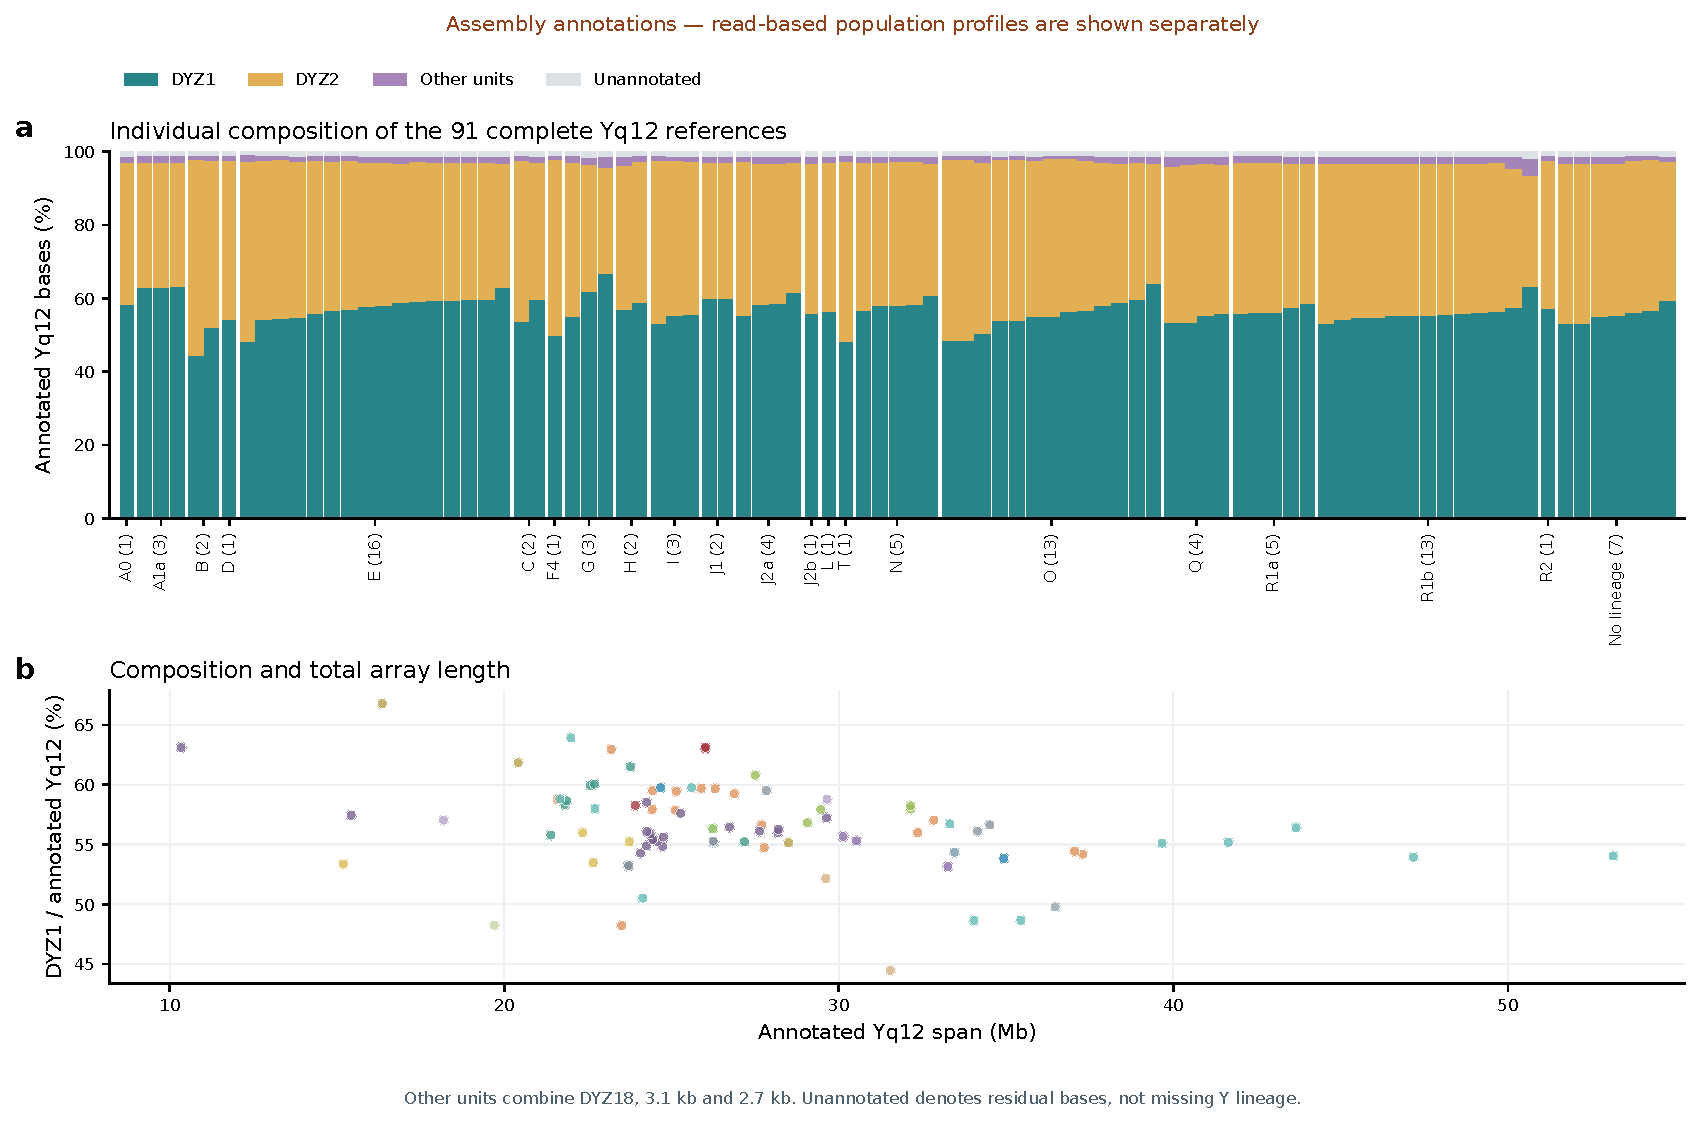
\includegraphics[width=\textwidth]{figures/figureS2_yq12_composition.pdf}
\caption{\textbf{Individual composition of complete Yq12 assembly references.} \textbf{a}, Per-individual composition of all 91 complete reference arrays, grouped by Y clade and sorted by DYZ1 fraction within each clade. Counts below groups give the number of references. The final seven references lack matching lineage metadata. DYZ1, DYZ2, other units (DYZ18, 3.1 kb and 2.7 kb) and residual unannotated bases sum to the annotated Yq12 span. \textbf{b}, DYZ1 fraction against annotated Yq12 span in the same 91 references. Colours denote broad Y lineages as in Supplementary Fig.~\ref{fig:map}; grey marks references without lineage metadata. The plot is descriptive and both axes use the same span. These are assembly annotations; the read-based population estimates are shown separately in Supplementary Fig.~\ref{fig:s-population}.}\label{fig:yq12-composition}
\end{figure}
\endgroup

\begingroup
\renewcommand{\thefigure}{S2}
\begin{figure}[tbp]
\centering
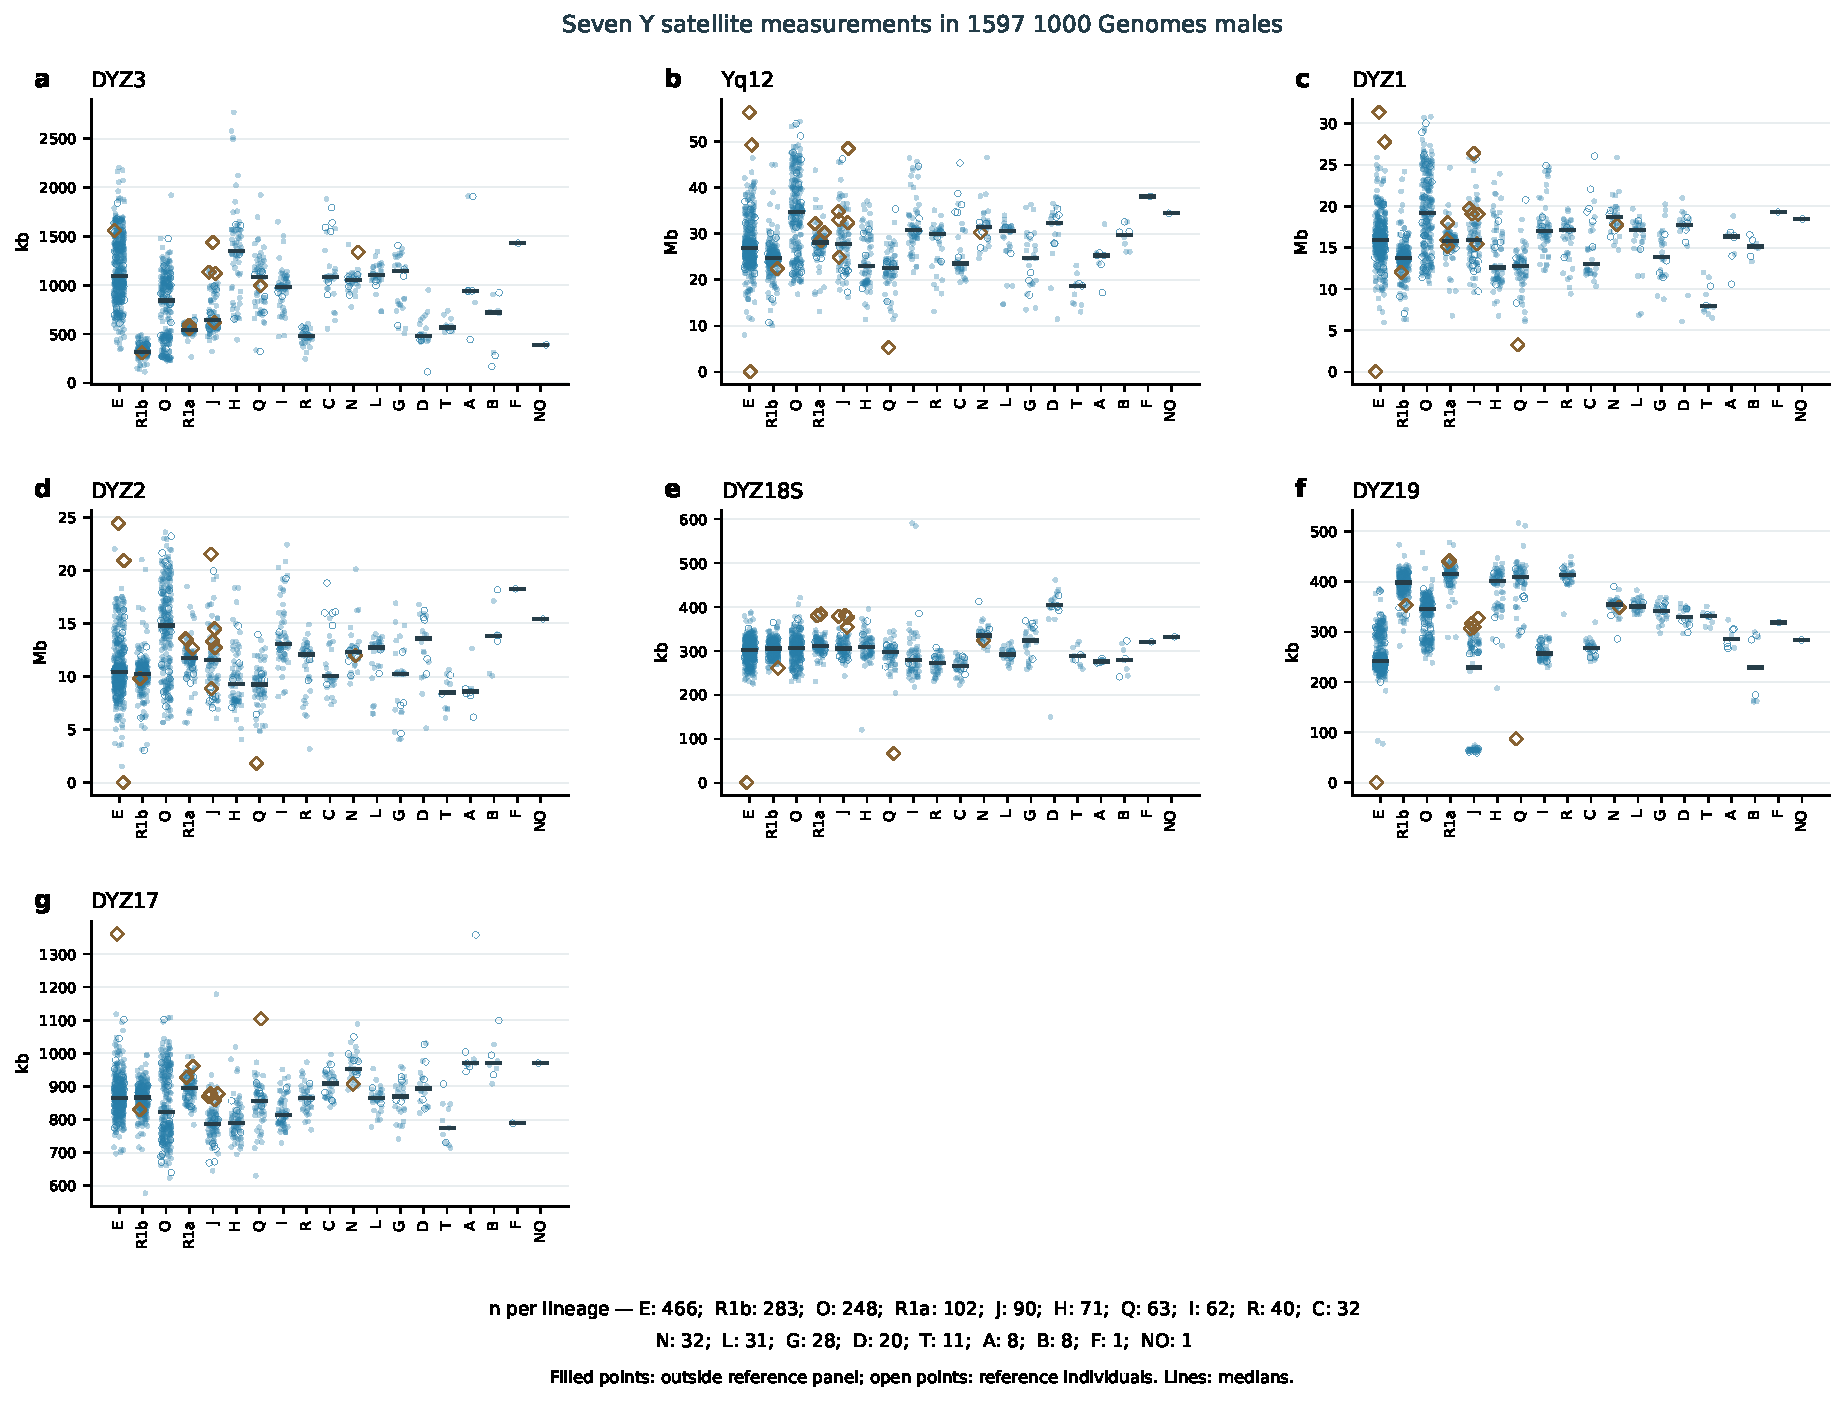
\includegraphics[width=\textwidth]{figures/figureS3_population.pdf}
\caption{\textbf{\vsette{Seven} satellite measurements across the analysed population.} \textbf{a--\vsette{g}}, Estimated lengths by broad Y lineage for all 1,597 males with estimates, retaining rare groups. Sample counts are listed below the panels; horizontal lines show medians. \textbf{\vsette{h}}, DYZ1 against DYZ2 estimated base-pair lengths, coloured by lineage. Filled circles have no reference assembly and open circles do. Diamonds identify arm-imbalanced or Yp-depleted profiles, excluded from medians and correlation estimates. Reference estimates can be in-sample. \vsette{Yq12 is the sum of DYZ1, DYZ2 and the rest of Yq12.} Uneven sampling and family dependence limit population-frequency interpretation.}\label{fig:s-population}
\end{figure}
\endgroup

\begingroup
\renewcommand{\thefigure}{S3}
\begin{figure}[tbp]
\centering
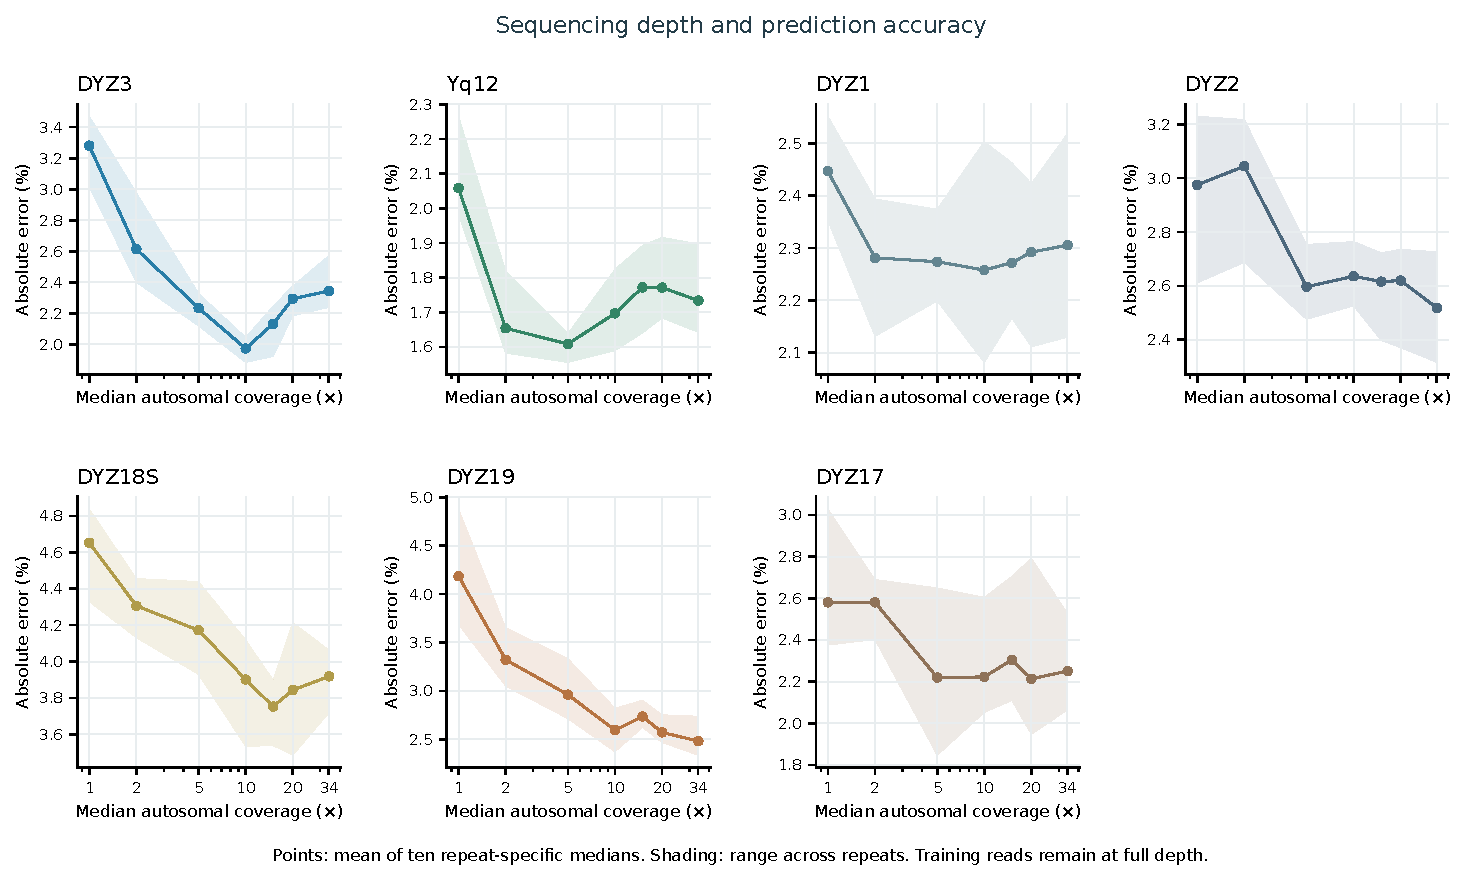
\includegraphics[width=\textwidth]{figures/figureS4_depth.pdf}
\caption{\textbf{Depth sensitivity of all \vsette{seven} targets.} Test reads are thinned to \vsette{20, 15, 10, 5, 2 and 1$\times$ of base coverage and shown with full depth (34.1$\times$)}, while training reads retain full depth. The x-axis gives median autosomal \vsette{base coverage}. Points show the mean of ten grouped-CV repeat-specific median absolute percentage errors, with shading showing their range. These ranges are not confidence intervals. Evaluated counts are \vsette{101 for DYZ3, 115 for DYZ19 and DYZ17, 80 for Yq12 and DYZ2, and 81 for DYZ1 and DYZ18S}. Downsampling reuses the same individuals, and its full-depth baseline matches the ten repeats in Table~\ref{tab:accuracy}.}\label{fig:s-depth}
\end{figure}
\endgroup

\begingroup
\renewcommand{\thefigure}{S4}
\begin{figure}[tbp]
\centering
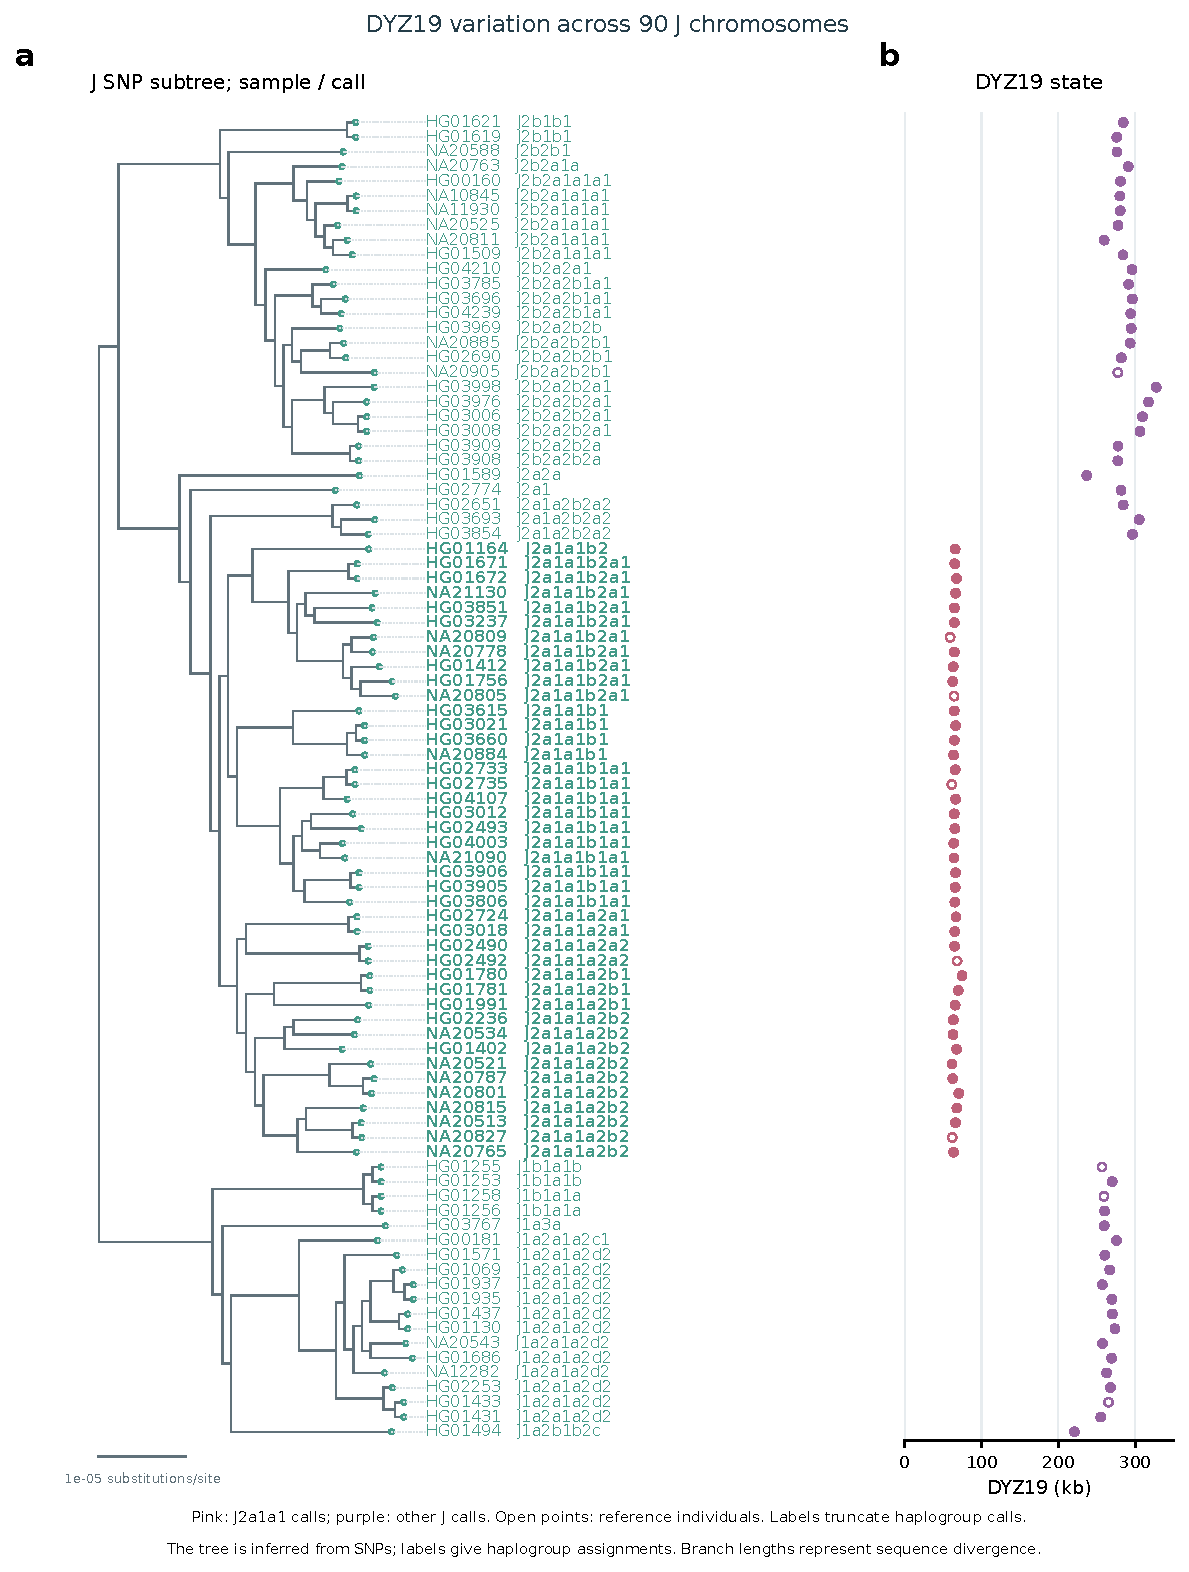
\includegraphics[width=.94\textwidth]{figures/figureS5_J_DYZ19.pdf}
\caption{\textbf{DYZ19 estimates aligned to the SNP tree of all 90 sampled J chromosomes.} \textbf{a}, Pruned tree retaining branch lengths; tips give sample identifiers and abbreviated ISOGG 2019 calls. \textbf{b}, Read-based DYZ19 estimates, with J2a1a1 calls in pink and other J calls in purple; open symbols mark males with reference assemblies. The short-state groups have distinct J2a1a1a and J2a1a1b calls within a single clade; J2a1a2 lies outside it. The tree is used descriptively; the number and timing of state transitions were not inferred.}\label{fig:j-dyz19}
\end{figure}
\endgroup

\clearpage
\begingroup
\renewcommand{\thefigure}{S5}
\begin{figure}[p]
\centering
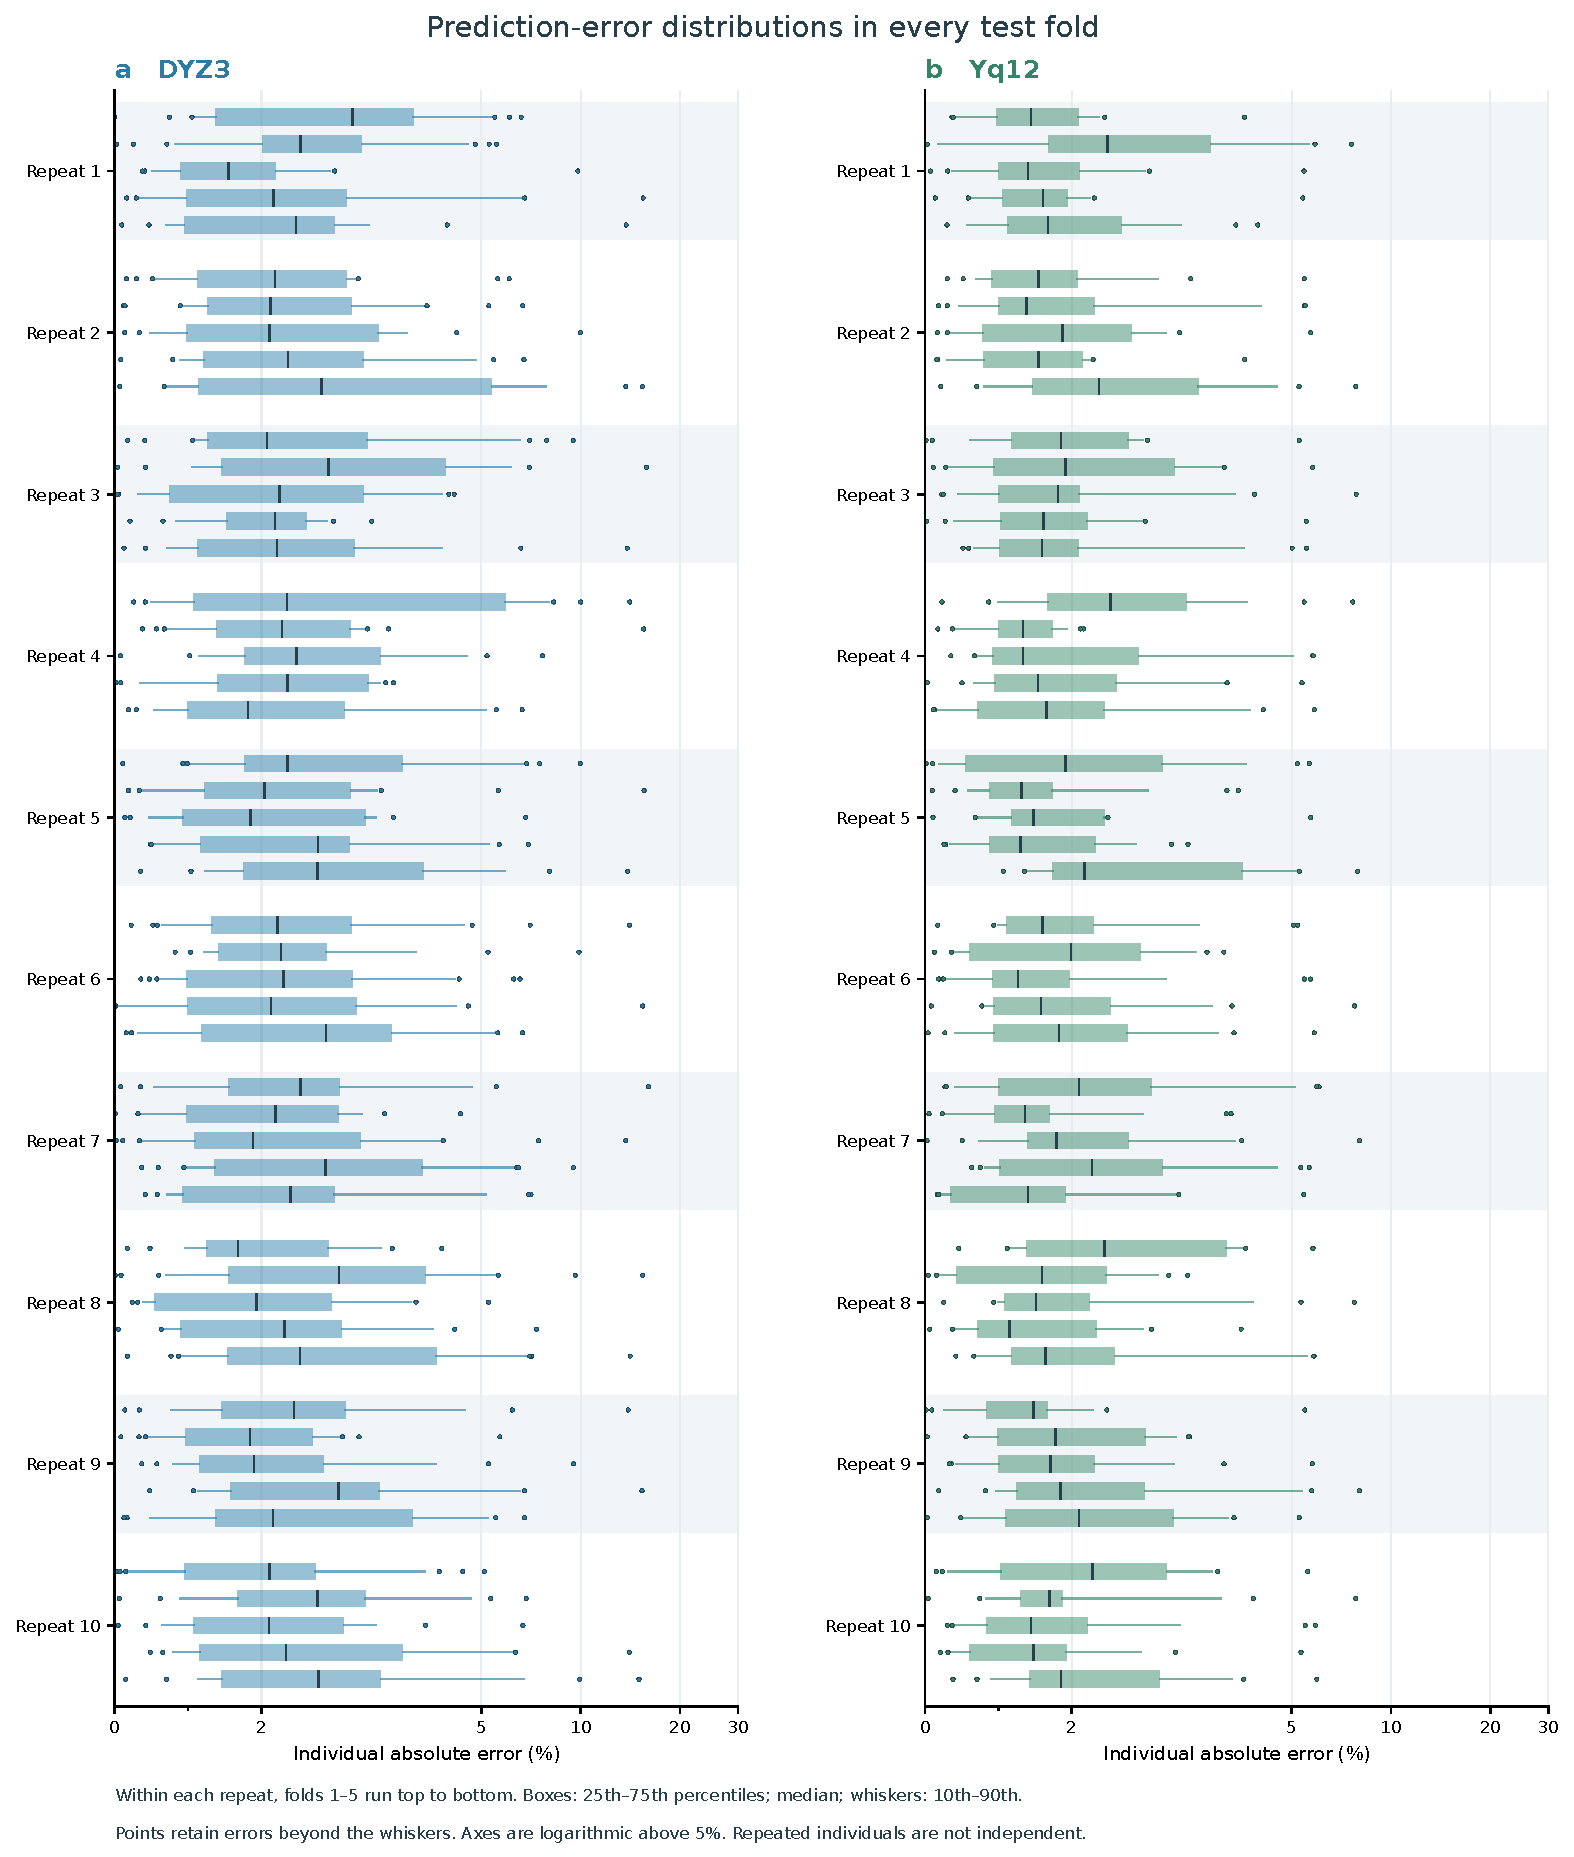
\includegraphics[page=1,width=\textwidth,height=.75\textheight,keepaspectratio]{figures/figureS6_cv_folds.pdf}
\caption{\textbf{Prediction-error variability in every cross-validation fold.} \textbf{a,b}, DYZ3 and Yq12. Each target shows all five test-fold distributions within each of ten repeats, with folds 1--5 running from top to bottom. Boxes span the 25th--75th percentiles, central lines mark medians and whiskers end at the 10th and 90th percentiles; points retain errors beyond the whiskers. Axes are linear through 5\% and logarithmic above. Repeated predictions of the same individual are not independent biological observations.}\label{fig:cv-folds}
\end{figure}
\endgroup

\clearpage
\begingroup
\renewcommand{\thefigure}{S5}
\begin{figure}[p]
\centering
\includegraphics[page=2,width=\textwidth,height=.75\textheight,keepaspectratio]{figures/figureS6_cv_folds.pdf}
\caption{\textbf{Prediction-error variability in every cross-validation fold (continued).} \textbf{c,d}, DYZ1 and DYZ2. Each target shows all five test-fold distributions within each of ten repeats, with folds 1--5 running from top to bottom. Boxes span the 25th--75th percentiles, central lines mark medians and whiskers end at the 10th and 90th percentiles; points retain errors beyond the whiskers. Axes are linear through 5\% and logarithmic above. Repeated predictions of the same individual are not independent biological observations.}
\end{figure}
\endgroup

\clearpage
\begingroup
\renewcommand{\thefigure}{S5}
\begin{figure}[p]
\centering
\includegraphics[page=3,width=\textwidth,height=.75\textheight,keepaspectratio]{figures/figureS6_cv_folds.pdf}
\caption{\textbf{Prediction-error variability in every cross-validation fold (continued).} \textbf{e,f}, DYZ18S and DYZ19. Each target shows all five test-fold distributions within each of ten repeats, with folds 1--5 running from top to bottom. Boxes span the 25th--75th percentiles, central lines mark medians and whiskers end at the 10th and 90th percentiles; points retain errors beyond the whiskers. Axes are linear through 5\% and logarithmic above. Repeated predictions of the same individual are not independent biological observations.}
\end{figure}
\endgroup

\clearpage
\begingroup
\renewcommand{\thefigure}{S5}
\begin{figure}[p]
\centering
\includegraphics[page=4,width=\textwidth,height=.75\textheight,keepaspectratio]{figures/figureS6_cv_folds.pdf}
\caption{\textbf{Prediction-error variability in every cross-validation fold (continued).} \textbf{g,h}, DYZ17 and the derived DYZ1:DYZ2 ratio; each ratio error pairs the component predictions of the same individual, repeat and fold. Each target shows all five test-fold distributions within each of ten repeats, with folds 1--5 running from top to bottom. Boxes span the 25th--75th percentiles, central lines mark medians and whiskers end at the 10th and 90th percentiles; points retain errors beyond the whiskers. Axes are linear through 5\% and logarithmic above. Repeated predictions of the same individual are not independent biological observations.}
\end{figure}
\endgroup
\clearpage

\clearpage

\clearpage

\begingroup
\renewcommand{\thefigure}{S6}
\begin{figure}[p]
\centering
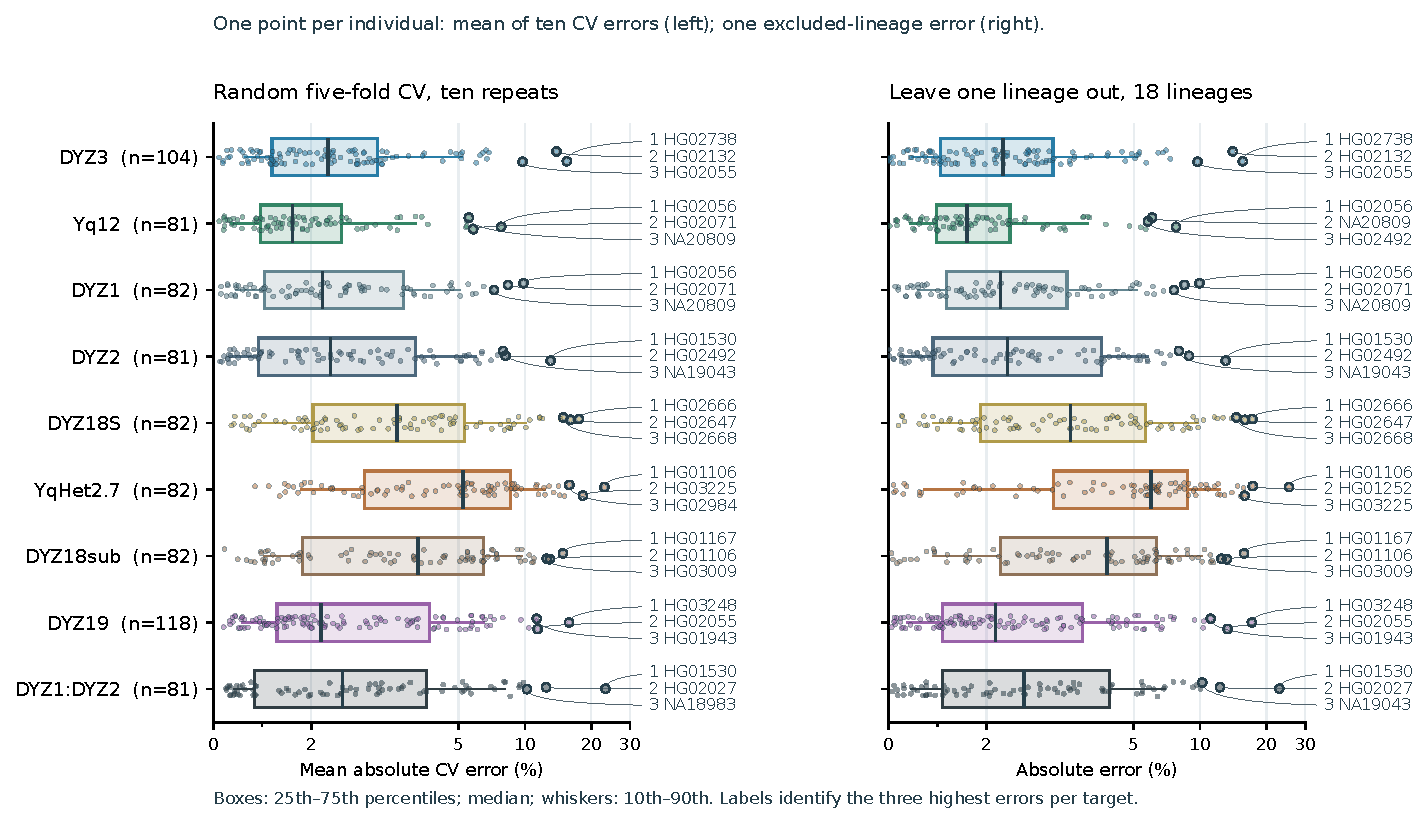
\includegraphics[width=\textwidth]{figures/figureS7_lineage_validation.pdf}
\caption{\textbf{Random cross-validation and exclusion of entire Y lineages.} Left: each point averages an individual's ten absolute percentage errors from family-grouped random five-fold CV. Right: each point is the individual's single absolute percentage error when its entire lineage is excluded from training, pooling all 18 excluded-lineage tests. Training also excludes any recorded family shared with test individuals. Each measurement has the same evaluated individuals in both panels; the final row is the derived DYZ1:DYZ2 ratio. Boxes span the 25th--75th percentiles, central lines mark medians and whiskers end at the 10th and 90th percentiles. All individual points are shown; labels identify the three largest displayed errors per target. Axes are linear through 5\% and logarithmic above.}\label{fig:lineage-validation}
\end{figure}
\endgroup
\clearpage

\clearpage
\begingroup
\renewcommand{\thefigure}{S7}
\begin{figure}[p]
\centering
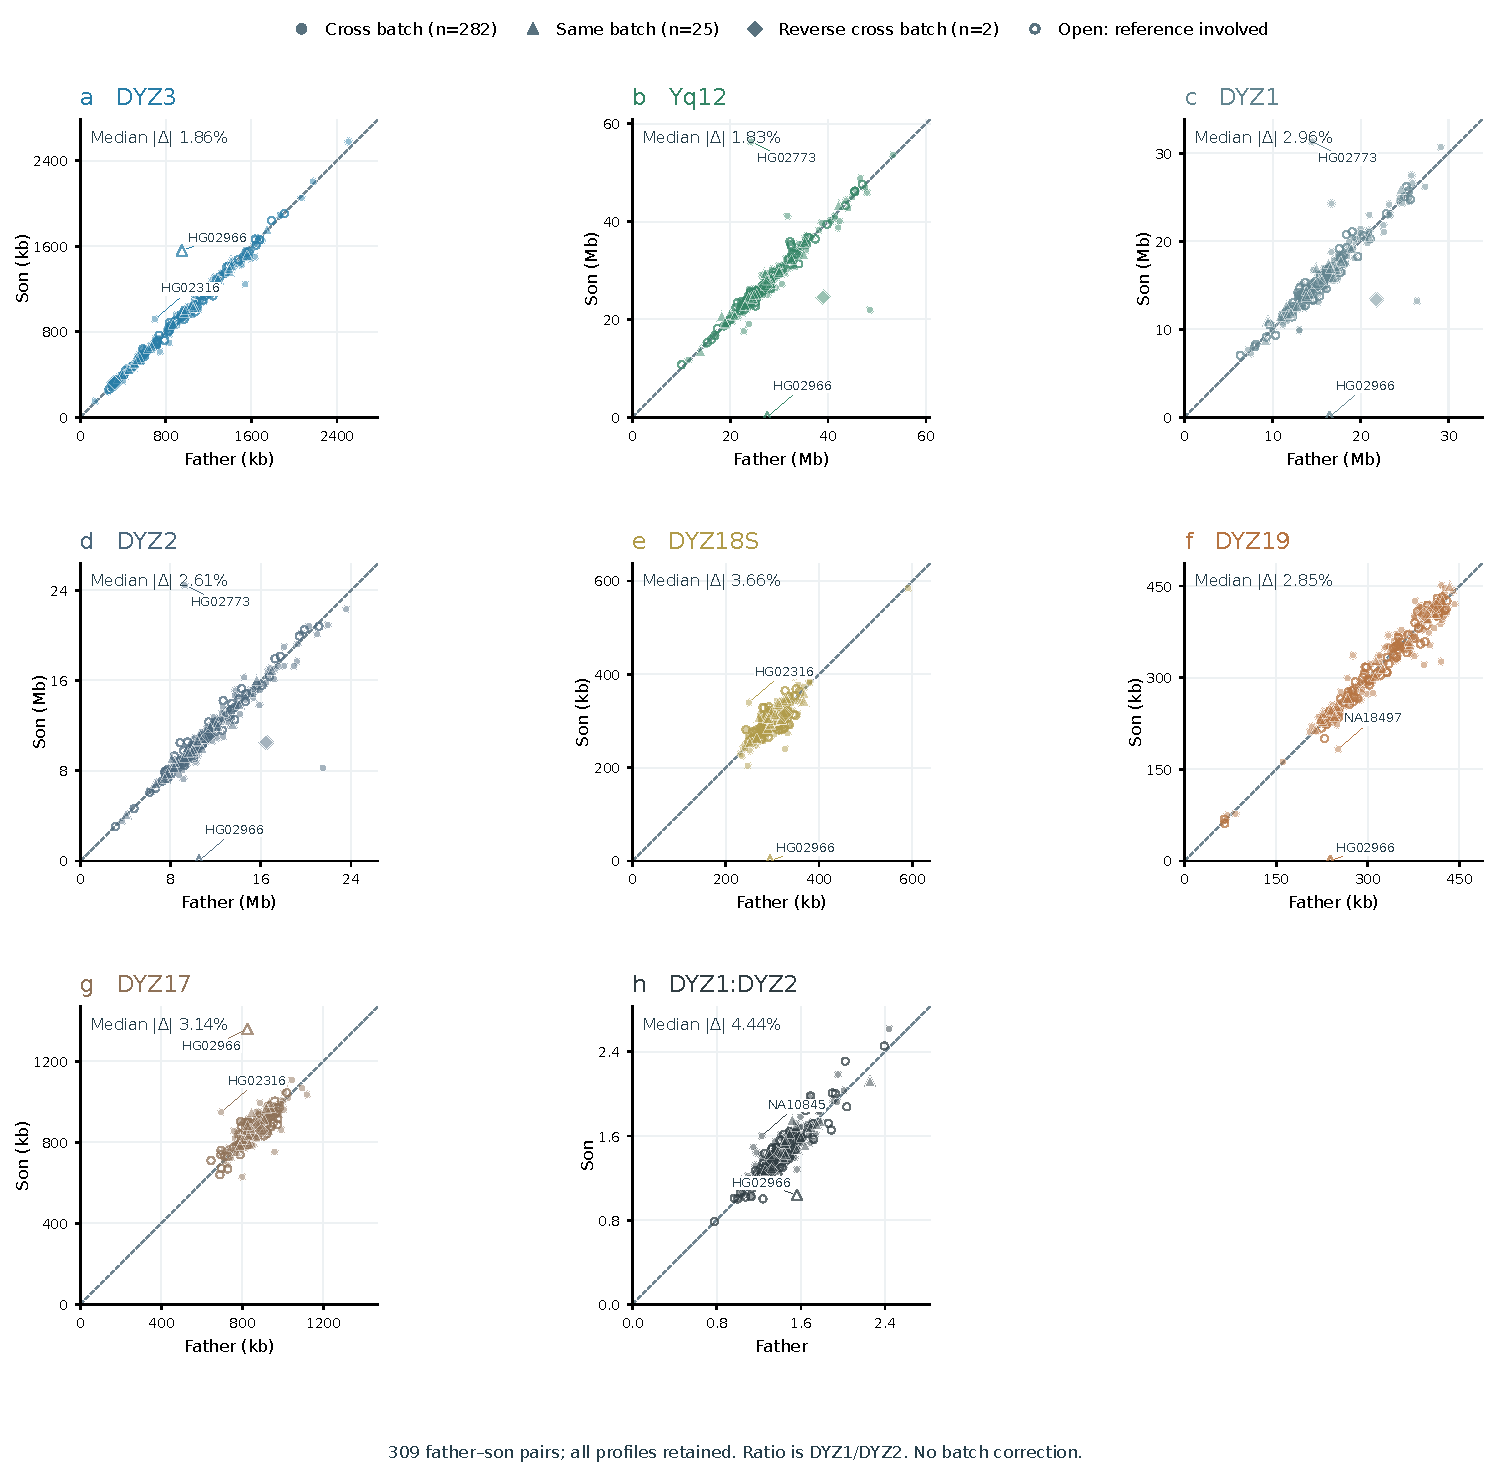
\includegraphics[page=1,width=\textwidth,height=.75\textheight,keepaspectratio]{figures/figureS8_all_pedigrees.pdf}
\caption{\textbf{Parent--offspring concordance for every satellite target and the DYZ1:DYZ2 length ratio.} \textbf{a--\vsette{h}}, All 309 pairs with complete estimates, shown for the \vsette{seven} targets and the derived ratio. Each point compares the parent's and offspring's estimates; diagonals mark equality and axes have matching limits. Colours match Fig.~\ref{fig:method}b. Shapes distinguish the 282 original-parent/additional-offspring pairs, 25 same-batch pairs and two reverse cross-batch pairs. Open points identify 78 pairs involving a male with a reference assembly (68 with a calibration male). Annotations give median absolute offspring/parent differences; labels identify offspring in the two pairs with the largest absolute percentage differences when these exceed 10\%. All complete profiles, including arm-imbalanced or Yp-depleted profiles, remain visible. No dosage cutoff or batch correction is applied. Targets use their indicated length units; the ratio is dimensionless. Pedigree pairs can share relatives and are not independent observations.}\label{fig:all-pedigrees}
\end{figure}

\endgroup

\clearpage
\begingroup
\renewcommand{\thefigure}{S7}
\begin{figure}[p]
\centering
\includegraphics[page=2,width=\textwidth,height=.75\textheight,keepaspectratio]{figures/figureS8_all_pedigrees.pdf}
\caption{\textbf{Parent--offspring concordance for every satellite target and the DYZ1:DYZ2 length ratio (continued).} \textbf{a--\vsette{h}}, Signed differences $100(\widehat L_{\mathrm{offspring}}/\widehat L_{\mathrm{parent}}-1)$ for the same measurements and pairs. For the ratio, $\widehat L$ denotes the individual's DYZ1:DYZ2 ratio. Batch contrasts are shown separately, including the two reverse-direction pairs. Points show every pair; horizontal segments span the 25th--75th percentiles, central marks and labels give medians. Difference axes are linear within $\pm5\%$ and logarithmic outside; their ranges retain all observations. Reference-involved pairs remain open. These differences combine technical variation, possible biological changes and flagged structural profiles; they are not mutation-rate estimates.}
\end{figure}
\endgroup

\begingroup
\renewcommand{\thefigure}{S8}
\begin{figure}[p]
\centering
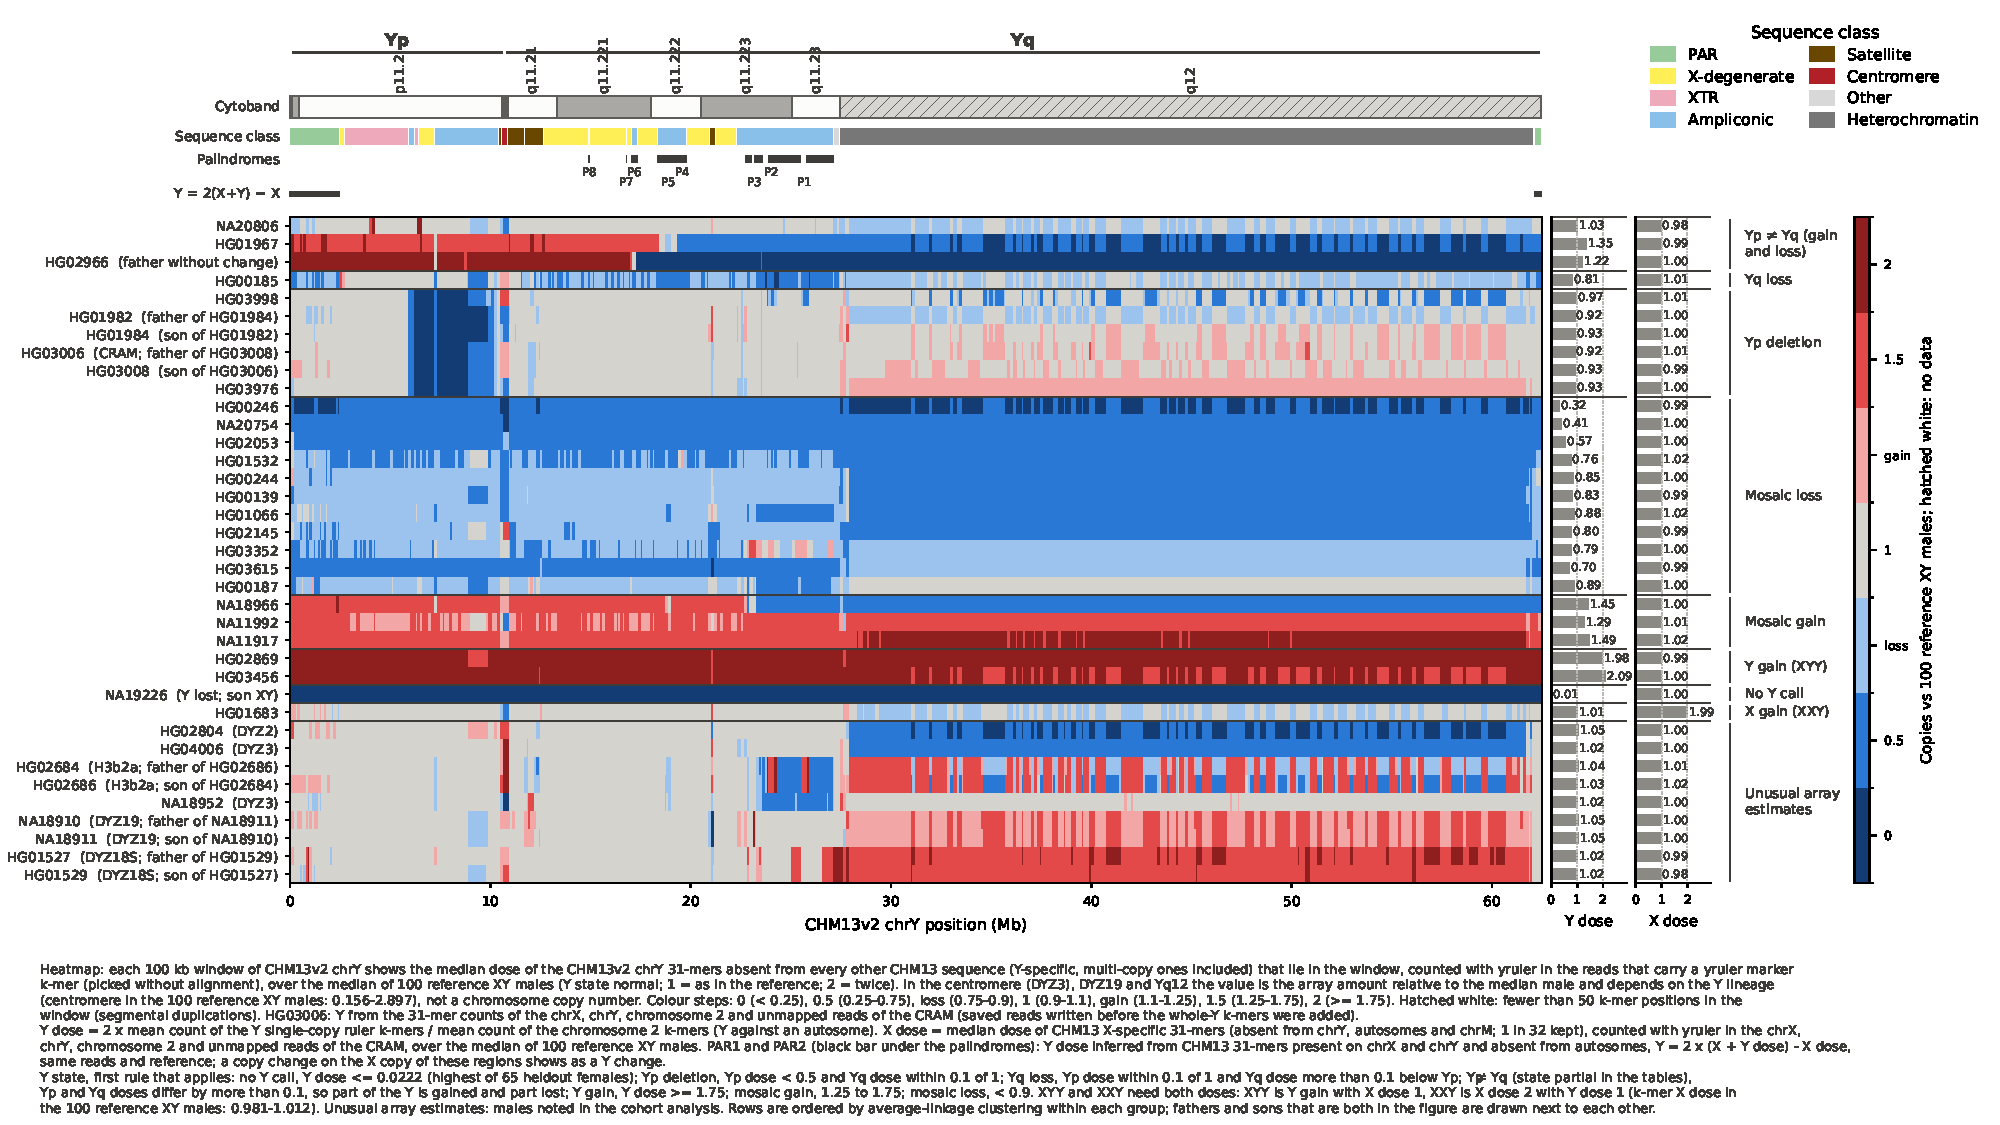
\includegraphics[width=\textwidth]{figures/figureS9_chrY_unusual_males.pdf}
\caption{\textbf{chrY profiles of 1000 Genomes males with an unusual Y state or array estimate.} Each row is one male and each column one of the 625 windows of 100 kb of CHM13v2 chrY; row labels give PAR2 doses of independent libraries where available; colours give, in seven steps, the median dose of the chrY 31-mers that occur on no other CHM13 sequence, relative to the median of 100 XY males with Y state normal. In PAR1 and PAR2 the Y dose is twice the dose of the 31-mers shared by chrX and chrY minus the X dose. Top: arms, cytobands, sequence classes \cite{Rhie2023} and palindromes. Right: Y dosage from the single-copy Y ruler and X dosage from 31-mers found only on chrX. Groups follow the Y state rules; parents and offspring that are both shown are drawn next to each other. In the centromere, DYZ19 and Yq12 the value is the array amount relative to the median male, not a chromosome copy number.}\label{fig:chrY-unusual}
\end{figure}

\endgroup
\begingroup
\renewcommand{\thefigure}{S9}
\begin{figure}[p]
\centering
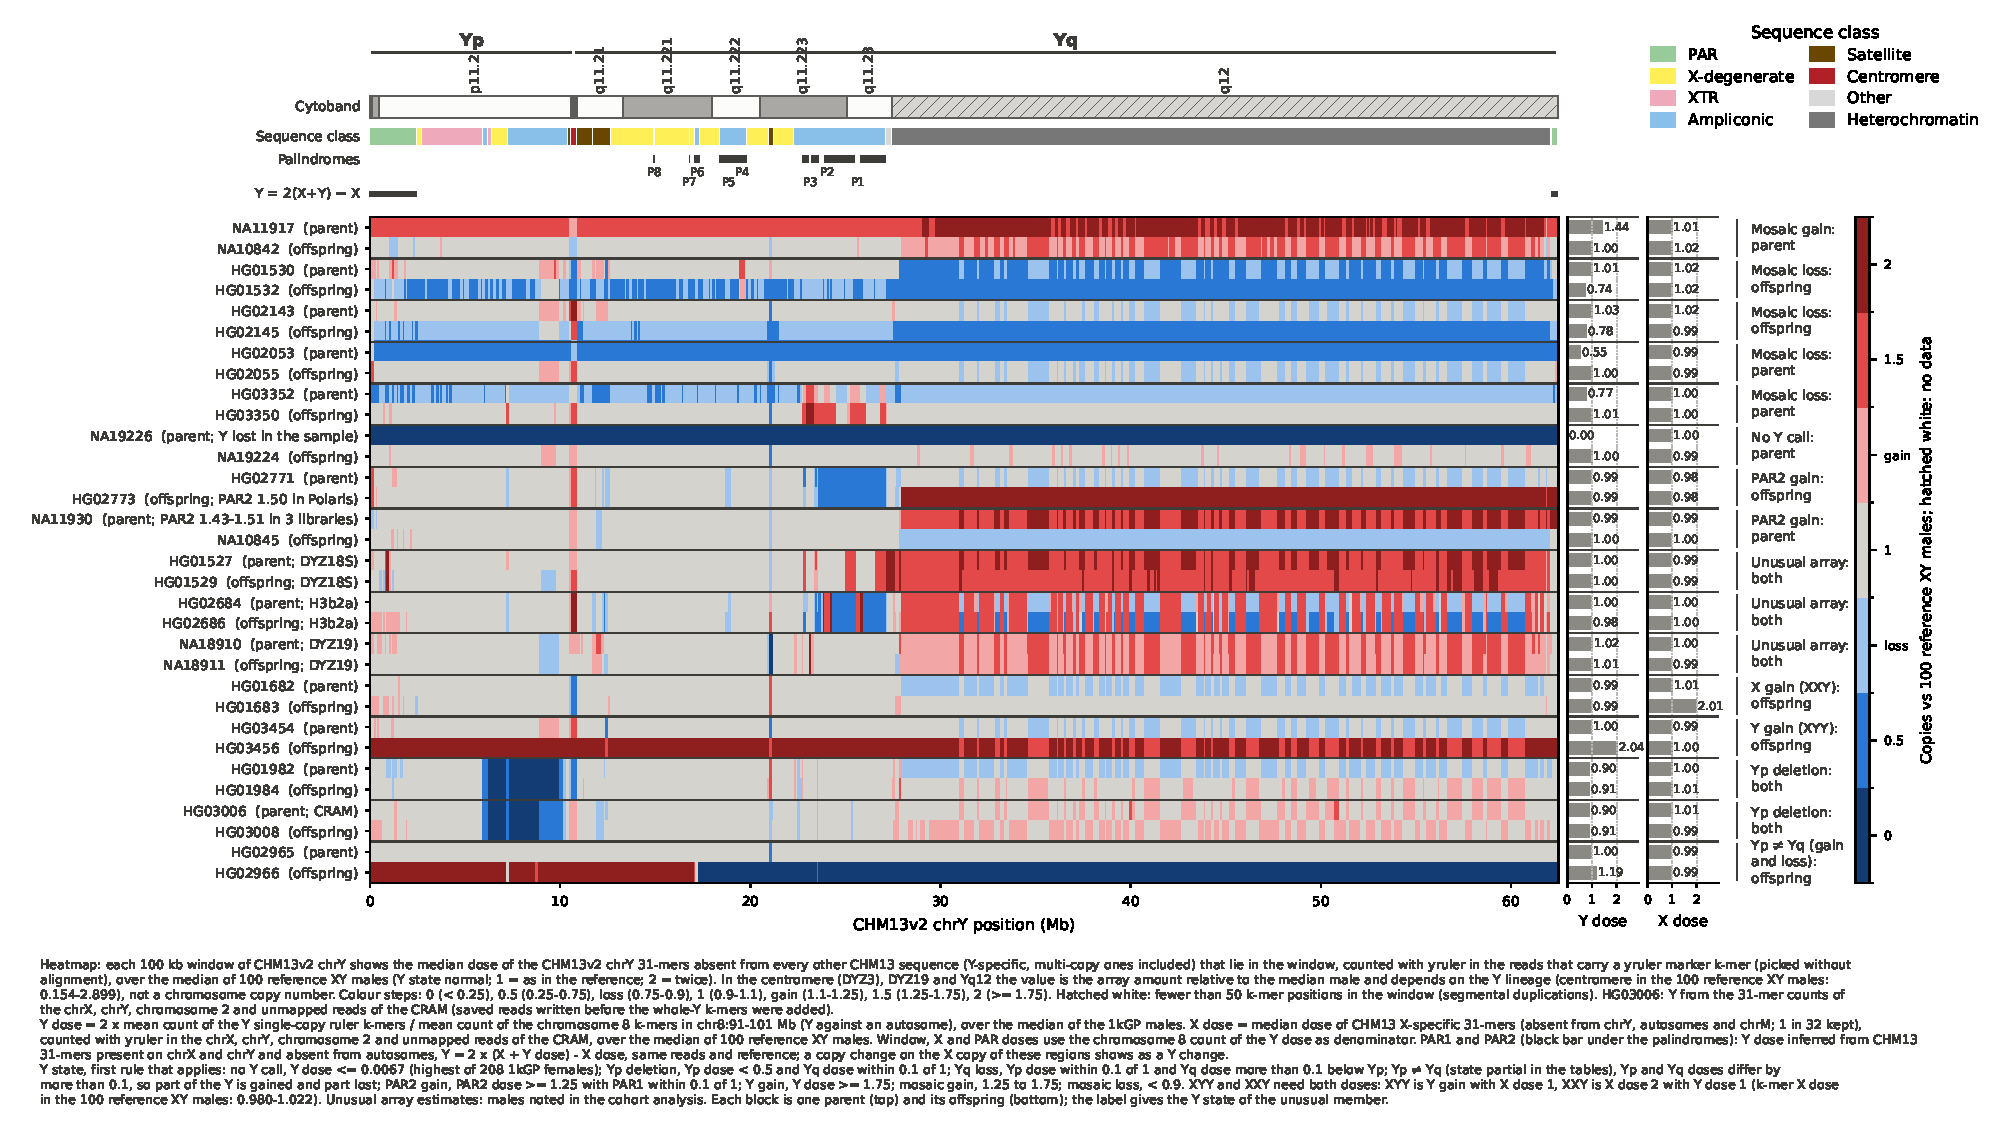
\includegraphics[width=\textwidth]{figures/figureS10_chrY_pairs.pdf}
\caption{\textbf{chrY profiles of the \vsette{16} parent--offspring pairs with an unusual member.} Panels as in Supplementary Fig.~\ref{fig:chrY-unusual}; in each block the parent is above its offspring, and the label gives the state of the unusual member.}\label{fig:chrY-pairs}
\end{figure}

\renewcommand{\thefigure}{S10}
\begin{figure}[tbp]
\centering
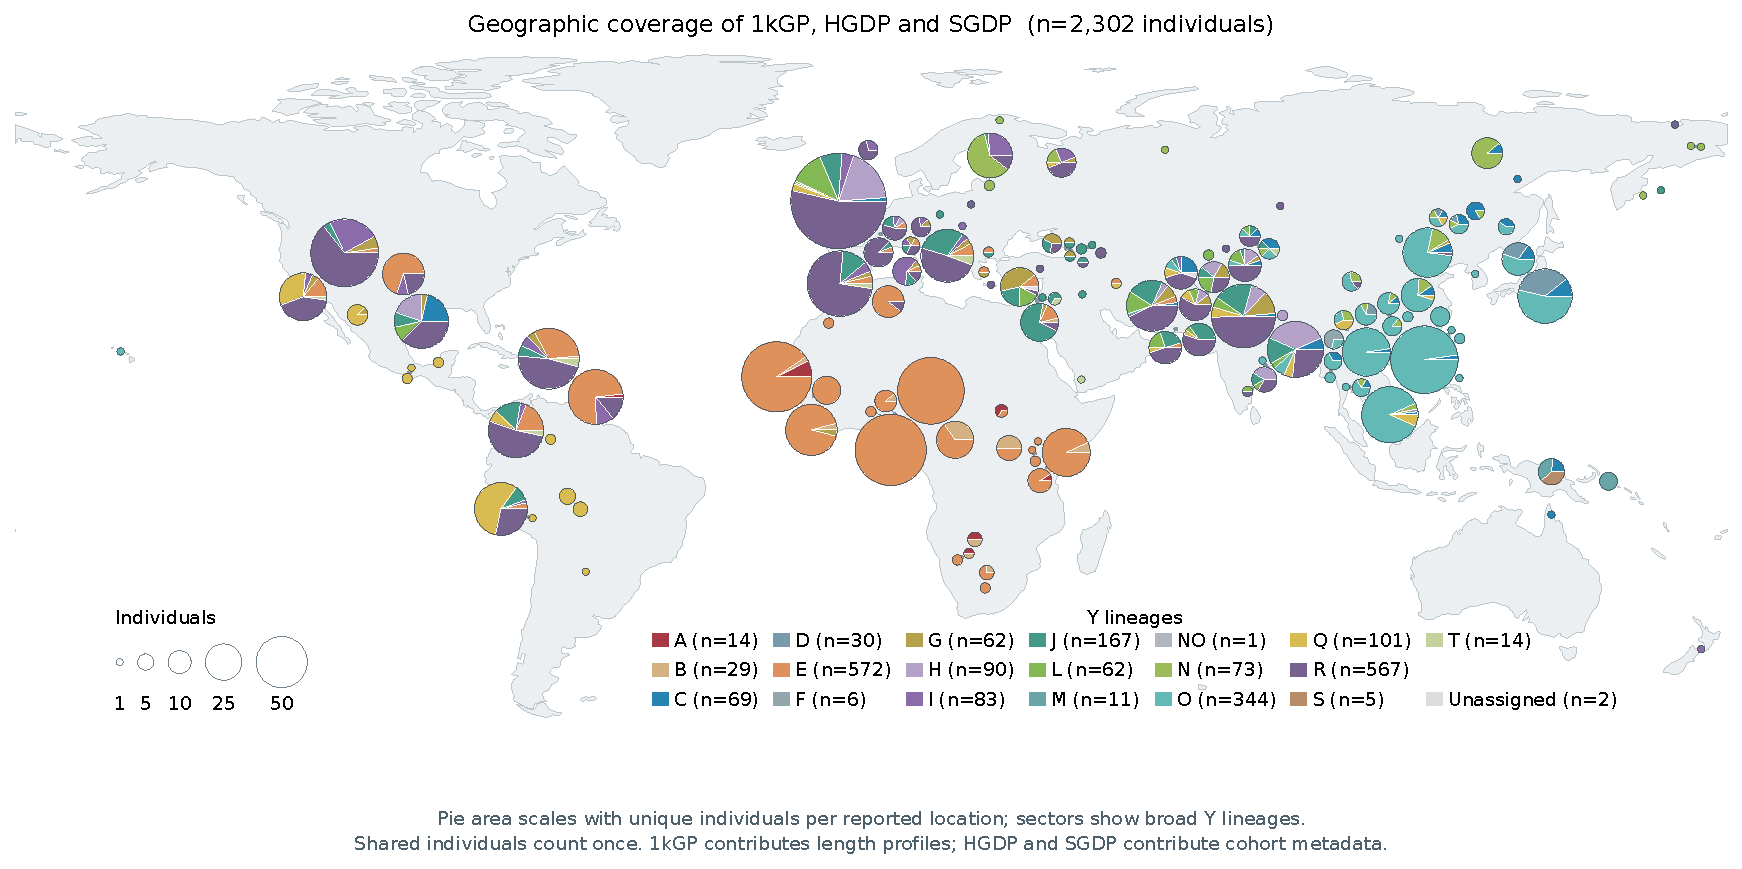
\includegraphics[width=\textwidth]{figures/cohort_world_map.pdf}
\caption{\textbf{Geographic coverage of the cohorts.} 1,597 1kGP individuals with estimates and HGDP/SGDP cohort manifests: 2,302 unique individuals after deduplication. Coordinates are cohort-reported population locations. Pie area scales with sample counts; sectors and legend counts show paternal Y lineages. Grey denotes two pending assignments; seven SGDP records reported as female and one additional record without Y signal are excluded (Online Methods).}\label{fig:map}
\end{figure}

\renewcommand{\thefigure}{S11}
\begin{figure}[tbp]
\centering
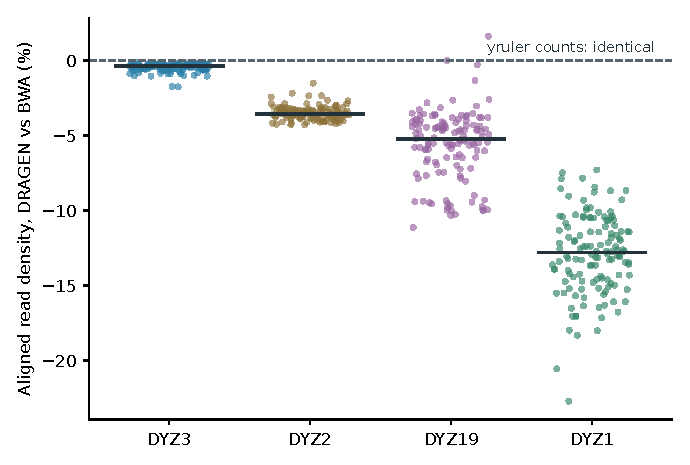
\includegraphics[width=.6\textwidth]{figures/figureS11_aligner_depth.pdf}
\caption{\textbf{Aligned read density depends on the aligner.} The same reads of 130 males, aligned with BWA and with DRAGEN 3.7.6. Each point is one male and shows the change in read density in the GRCh38 array block relative to chrY:14.5--15.5 Mb; bars show medians. The dashed line marks no change, as obtained for the yruler counts.}\label{fig:aligner}
\end{figure}
\endgroup


\clearpage
